\documentclass[11pt]{article}

% Any percent sign marks a comment to the end of the line

% Every latex document starts with a documentclass declaration like this
% The option dvips allows for graphics, 12pt is the font size, and article
%   is the style

\usepackage[pdftex]{graphicx}
\usepackage[utf8]{inputenc}
\usepackage{url}
\usepackage{titling}
\usepackage{lipsum}
\usepackage{geometry}
\usepackage{multicol}
\usepackage{setspace}
\usepackage{svg}
\usepackage{amsmath}
\usepackage{float}
\usepackage{url}
\usepackage{listings}


% These are additional packages for "pdflatex", graphics, and to include
% hyperlinks inside a document.

%\setlength{\oddsidemargin}{0.25in}
%\setlength{\textwidth}{6.5in}
%\setlength{\topmargin}{0in}
%\setlength{\textheight}{8.5in}
\setlength{\columnsep}{10mm}
\setlength{\droptitle}{-7em}   % This is your set screw
\graphicspath{{img/}}
%\onehalfspacing


\geometry{
	a4paper,
	total={170mm,257mm},
	left=25mm,
	top=30mm,
	right=25mm,
	bottom=35mm,
}
% These force using more of the margins that is the default style

\begin{document}

% Everything after this becomes content
% Replace the text between curly brackets with your own

\title{\huge \textbf{Movie Recommendation\\ Using Latent Factor Models}}
\author{\Large Mustafa Onur Eken\\[1mm] Bogazici University - CmpE 462}
\date{\today}

% You can leave out "date" and it will be added automatically for today
% You can change the "\today" date to any text you like
\maketitle
\begin{center}
	\section*{\large Abstract}
	\textit{Recommender systems are nearly obligatory in every platform where a type of content is served to users as long as conversion rates are concerned in perspective of bussiness owners. In like manner customers also benefit from since they discover interesting content at a faster rate. There have been different proposals to tackle problem of recommendation. In this project, we will implement a recent technique namely, latent factor models, go through the results we obtained and discuss strengths and weaknesses of it.}	
\end{center}
\vspace{10mm}


\begin{multicols}{2}	
	\section{Introduction}
	Content-based filtering and collaborative filtering are two main approaches used in practice nowadays to overcome the problem of item recommendation to users. In spite of content-based filtering, collaborative filtering does not make use of any domain-specific features about items and users, instead it attempts to find similarities between users and items only by examining the given ratings.
	

		
	Latent factor models assume that there are a number of characteristics of items and users. If characteristics of a user and an item are aligned then a user tend to like that item. Building on this assumption, we can discover the characteristics of users and items through factorizing the rating matrix, $R$, into two other matrices $U_{mxk}$ and $I_{nxk}$ such that $R = U I^T$.	 \\
	\begin{center}
		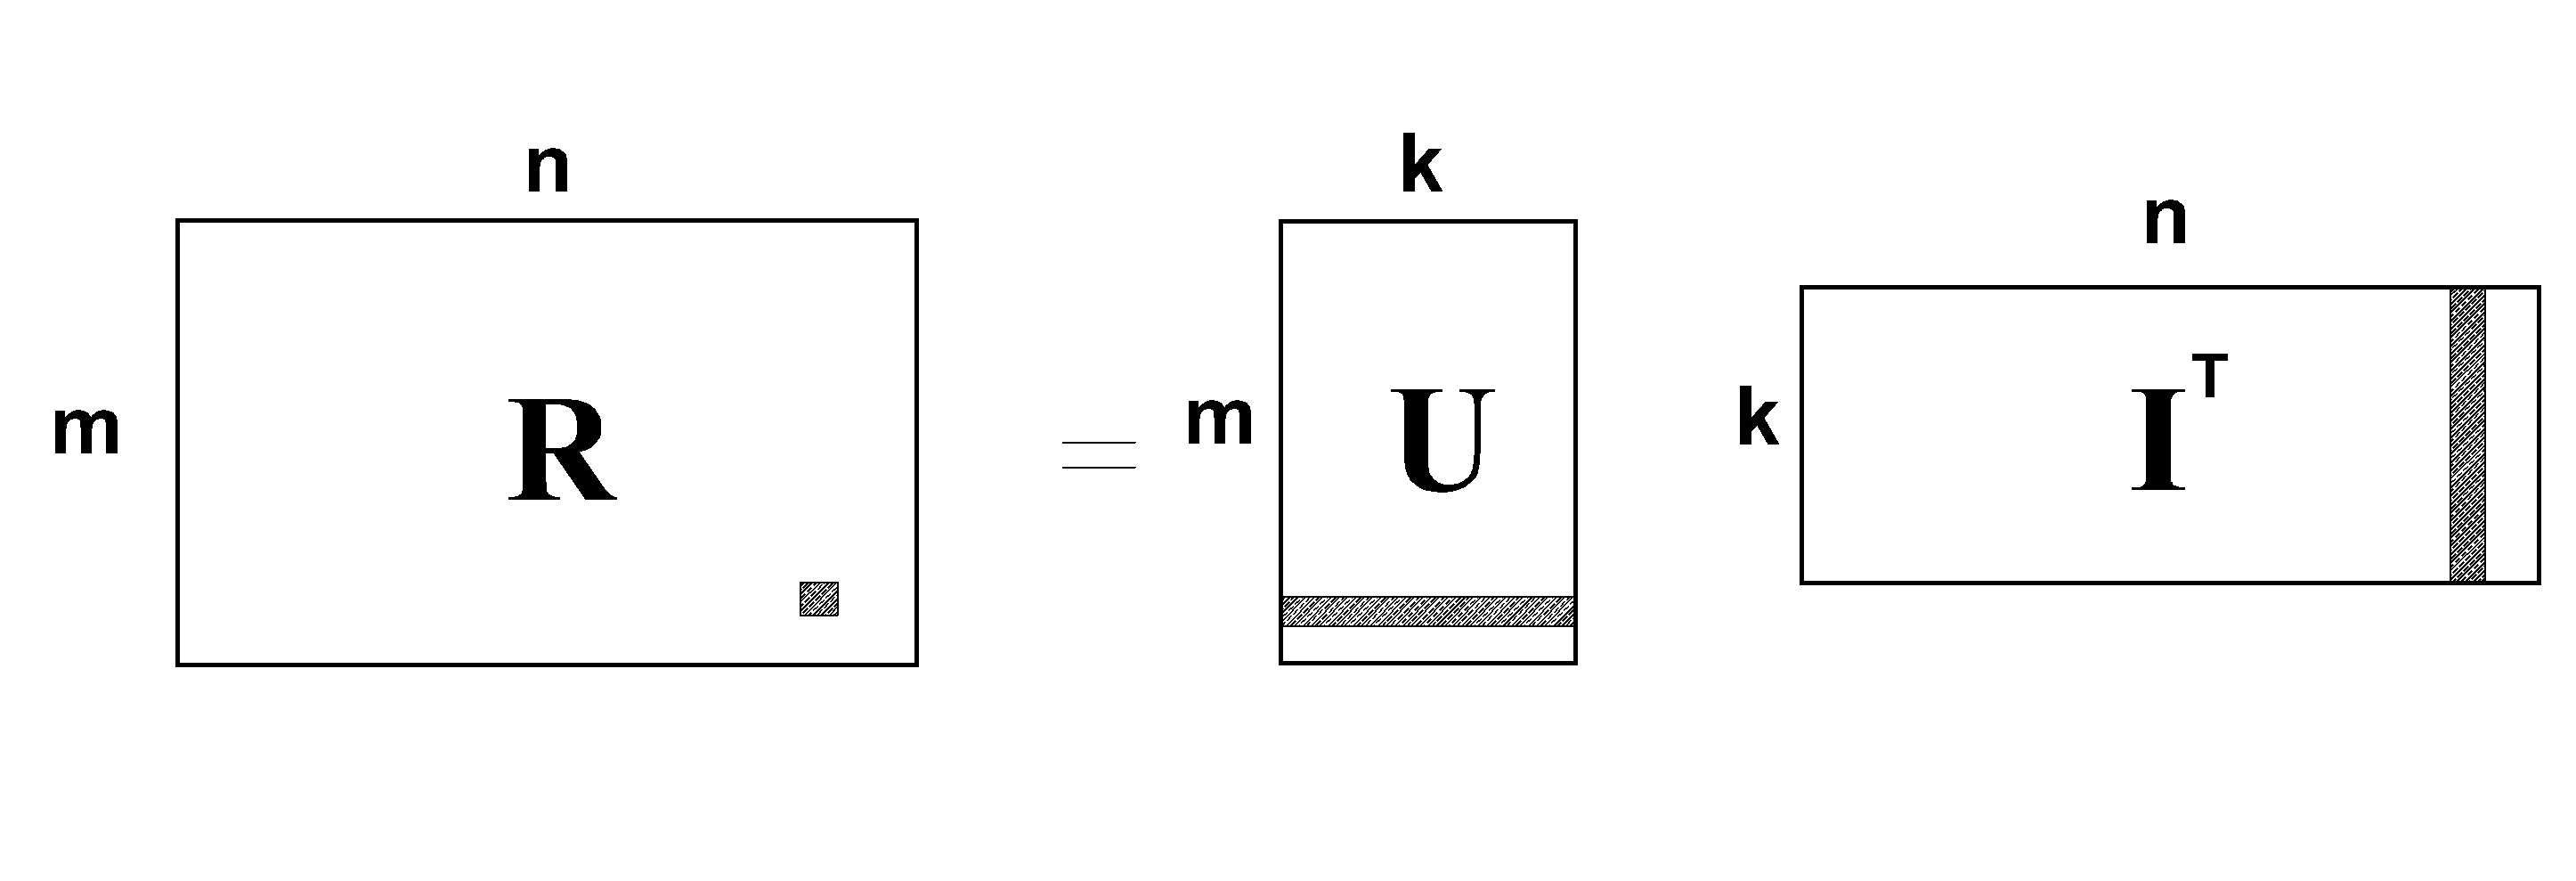
\includegraphics[width=0.8\columnwidth]{buff5/decomp}\\		
		\textit{Where $k$ is the number of latent factors.}
	\end{center}	
	Since matrix $R$ has missing entries computing SVD with common methods is not possible. There has been several proposals to compute this decomposition \cite{mnih,koren}. In this project we are going to implement computation of this factorization via 1) Stochastic gradient descent 2) Alternating least squares. In the following section we will briefly tell some important points in implementation of these algorithms. On the third section we will discuss the results we have obtained. Afterwards we will review strengths, weaknesses of matrix factorization methods and by point our some possible improvements. You can find the full source code in the appendices section.
		
	\section{Approach}
		\subsection{Data}
		In this project we use the well known \textit{MovieLens 100k} dataset where 943 people, 1682 movies and 100,000 ratings exist. Size of training data is 80,000 and the size of test data is 20,000. The rating density corresponds to 5.04\% when training data is considered. Although dataset contains item and user specific information such as occupation of a user, genre of a movie etc. we are not going to exploit them as they are irrelevant to basic version of latent factor models.
		
		\subsection{SGD}
		One way to find matrices $U$ and $I$ is by applying stochastic gradient descent. We initialize the matrices $U$ and $I$ randomly. We compute error based on one instance at a time. Lets denote $i$th row of matrix $U$ as $p_i$ and adjoint of $j$th row of matrix $I$ as $q_j$. In addition denote the difference between desired output and prediction as $d_{ij} = r_{ij} - \hat{r}_{ij}$
		\subsubsection{Plain}		
			In this model, prediction, error and update are calculated as follows:						
			$$\hat{r}_{ij} = p_i q_j$$ 
			$$d_{ij} = r_{ij} - p_i q_j$$
			$$e_{ij} = (d_{ij})^2 = (r_{ij} - p_i q_j)^2$$
			$$\frac{\partial e_{ij}}{\partial p_i} = -2 d_{ij} q_j$$
			$$\frac{\partial e_{ij}}{\partial q_j} = -2 d_{ij} p_i$$	
			$$p'_i = p_i + \eta d_{ij} q_j$$			
			$$q'_j = q_j + \eta d_{ij} p_i$$			
		\subsubsection{Plain + Regularization}		
			In this model, prediction, error and update are calculated as follows:						
			$$\hat{r}_{ij} = p_i q_j$$ 
			$$d_{ij} = r_{ij} - p_i q_j$$
			$$e_{ij} = (d_{ij})^2 + \lambda (\|p_i\|^2 + \|q_j\|^2)$$
			$$\frac{\partial e_{ij}}{\partial p_i} = -2 d_{ij} q_j + 2\lambda p_i$$
			$$\frac{\partial e_{ij}}{\partial q_j} = -2 d_{ij} p_i + 2\lambda q_j$$	
			$$p'_i = p_i + \eta (d_{ij} q_j - \lambda p_i)$$			
			$$q'_j = q_j + \eta (d_{ij} p_i - \lambda q_j)$$			
		\subsubsection{Plain + Biases}		
			In this model, we take user and movie specific biases into account to enhance the accuracy furthermore \cite{koren}. It's well known that some users tend to rate high on average while some other users rate. In like manner some movies are rated higher than others. In this sense bias of a movie represent how much users liked it. Here, $\mu$ is the mean of all ratings, $u_i$ is the bias of $i$th user and $m_j$ is the bias of $j$th movie. Prediction, error and update are calculated as follows:						
			$$\hat{r}_{ij} = \mu + u_i + m_j + p_i q_j$$ 
			$$d_{ij} = r_{ij} - \mu-+ u_i - m_j - p_i q_j$$
			$$e_{ij} = (r_{ij} - \mu-+ u_i - m_j - p_i q_j)^2$$
			$$\frac{\partial e_{ij}}{\partial p_i} = -2 d_{ij} q_j$$
			$$\frac{\partial e_{ij}}{\partial q_j} = -2 d_{ij} p_i$$	
			$$\frac{\partial e_{ij}}{\partial u_i} = -2 d_{ij} $$
			$$\frac{\partial e_{ij}}{\partial m_j} = -2 d_{ij} $$	
			$$p'_i = p_i + \eta d_{ij} q_j$$			
			$$q'_j = q_j + \eta d_{ij} p_i$$				
			$$u'_i = u_i + \eta d_{ij}$$			
			$$m'_j = m_j + \eta d_{ij}$$				
		\subsubsection{Plain + Regularization + Biases}		
			If we combine all, we get the following definitions for prediction, error and update:
			$$\hat{r}_{ij} = \mu + u_i + m_j + p_i q_j$$ 
			$$d_{ij} = r_{ij} - \mu-+ u_i - m_j - p_i q_j$$
			$$e_{ij} = (d_{ij})^2 + \lambda (\|p_i\|^2 + \|q_j\|^2 + u^2_i + m^2_j)$$
			$$\frac{\partial e_{ij}}{\partial p_i} = -2 d_{ij} q_j + 2 \lambda p_i$$
			$$\frac{\partial e_{ij}}{\partial q_j} = -2 d_{ij} p_i + 2 \lambda q_j$$	
			$$\frac{\partial e_{ij}}{\partial u_i} = -2 d_{ij} + 2 \lambda u_i$$
			$$\frac{\partial e_{ij}}{\partial m_j} = -2 d_{ij} + 2 \lambda m_j$$	
			$$p'_i = p_i + \eta (d_{ij} q_j - \lambda p_i)$$			
			$$q'_j = q_j + \eta (d_{ij} p_i - \lambda q_j)$$			
			$$u'_i = u_i + \eta (d_{ij}  - \lambda u_i)$$			
			$$m'_j = m_j + \eta (d_{ij}  - \lambda m_j)$$			
	\subsection{ALS}
		The key idea in alternating least squares somewhat similar to SGD. Instead of adjusting matrices $U$ and $I$ instances by instance, we fix one of them and solve least squares for the other one.
		$$U I^T = R$$
		Fix $U$ and solve for $I^T$. Then fix $I^T$ then solve for $U$. Repeat this until convergence. If one desires to use MATLAB's $\setminus$ operator for solving least squares, a re-formulation of matrices $U$ and $I^T$ is needed. An example of a toy set up would be as following:
		\[
		\begin{bmatrix}
			x_{11}	& ?  \\
			x_{21}  & x_{22}
		\end{bmatrix}		
		= 		
		\begin{bmatrix}
		a_{11}	& a_{12}  \\
		a_{21}  & a_{22}
		\end{bmatrix}		
		*
		\begin{bmatrix}
		b_{11}	& b_{12}  \\
		b_{21}  & b_{22}
		\end{bmatrix}		
		\]		
		\[
		\begin{bmatrix}
		x_{11}	\\
		x_{21} \\
		x_{22}
		\end{bmatrix}		
		= 
		\begin{bmatrix}
		a_{11} & a_{12} & 0 		& 0 \\
		a_{21} & a_{22} & 0 		& 0    \\
		0		  & 0		  & a_{21} & a_{22}
		\end{bmatrix}		
		*
		\begin{bmatrix}
		b_{11} \\
		b_{21} \\
		b_{12} \\
		b_{22}
		\end{bmatrix}		
		\]
		
		Here we find  $b$ values by solving $x = A_m b$. (I.e. $A_m \setminus x$ in MATLAB) The same formulation must be done on the second matrix as well. ALS execution time is unfavorable \cite{koren} compared to SGD unless 
		\begin{itemize}
			\setlength\itemsep{1mm}
			\item Parallelization is possible.
			\item Data is not sparse.
		\end{itemize}
		
			
		
		
		
%	\begin{figure*}[!ht]
%		\centering
%		\includegraphics[width=1.7\wi]{user_sgd}
%		\caption{djlaskjda}
%		\label{1}
%	\end{figure*}
%	\begin{figure*}[!ht]
%		\centering
%		\includegraphics[width=1.7\wi]{user_als}
%		\caption{djlaskjda}
%		\label{2}
%	\end{figure*}
%	\begin{figure*}[!ht]
%		\centering
%		\includegraphics[width=1.7\wi]{mov_sgd}
%		\caption{djlaskjda}
%		\label{3}
%	\end{figure*}
%	\begin{figure*}[!ht]
%		\centering
%		\includegraphics[width=1.7\wi]{mov_als}
%		\caption{djlaskjda}
%		\label{4}
%	\end{figure*}
	
	
	
	
	\section{Results \& Discussion}
	We have implemented both algorithms (biases and regularization terms are not included in ALS) and executed on 1)\textit{Hand-crafted toy data} 2)\textit{MovieLens 100k data}. Find output plots and interpretation of them in the following pages. 
	
	Although both ALS and SGD worked just fine on toy data, ALS became infeasible when MovieLens data is given as input. Therefore, plots associated with MovieLens data are generated as a result of SGD algorithm only.
	
	For illustration purposes we first run the algorithms on "full" toy data (i.e. no missing entries) assuming two latent factors. Since the rating matrix is full we also executed SVD algorithm to validate results of other algorithms, SGD and ALS. When we plot the values of latent factors for movies and users we see nice clusters in accordance with the generation of the toy data. This vaguely confirms that the model can indeed find hidden patterns in the data. We also trained the model using one latent factor to see if clusters are distinguishable. Unfortunately there were no apparent separate clusters. It indicates that one factor is not enough to explain/approximate the given data.
	
	We used a small, fixed learning rate in SGD instead of an adaptive learning rate because the dataset was not gigantic and execution times were reasonable in nearly all settings of parameters. 
		
	\section{Conclusion}
	As seen on the plots and tables, latent factor models are rather accurate in finding recommendations. When data density is high (see tests on toy data) the results are nearly perfect. When it is sparse (see tests on MovieLens data) we can say that it is satisfactory. It is neat that when data can be explained with a few latent factors we can visualize it and expose clusters.
	
	This project can be improved by attacking the problem of finding optimal values for parameters such as number of latent factors, regularization coefficient in order to minimize error. Furthermore, it could have been nice to implement ALS to work on a parallel platform and see the training results on the real data.
	
	

	\bibliography{refs}
	\bibliographystyle{unsrt}
\end{multicols}
\vspace{15mm}

	\def \wi {0.75\columnwidth}
	
	\def \wiq {0.70\columnwidth}	
	\begin{center}
		\Large \textbf{\underline{Tests on Toy Data}}
	\end{center}

	
	\begin{figure}[H]
		\centering		
		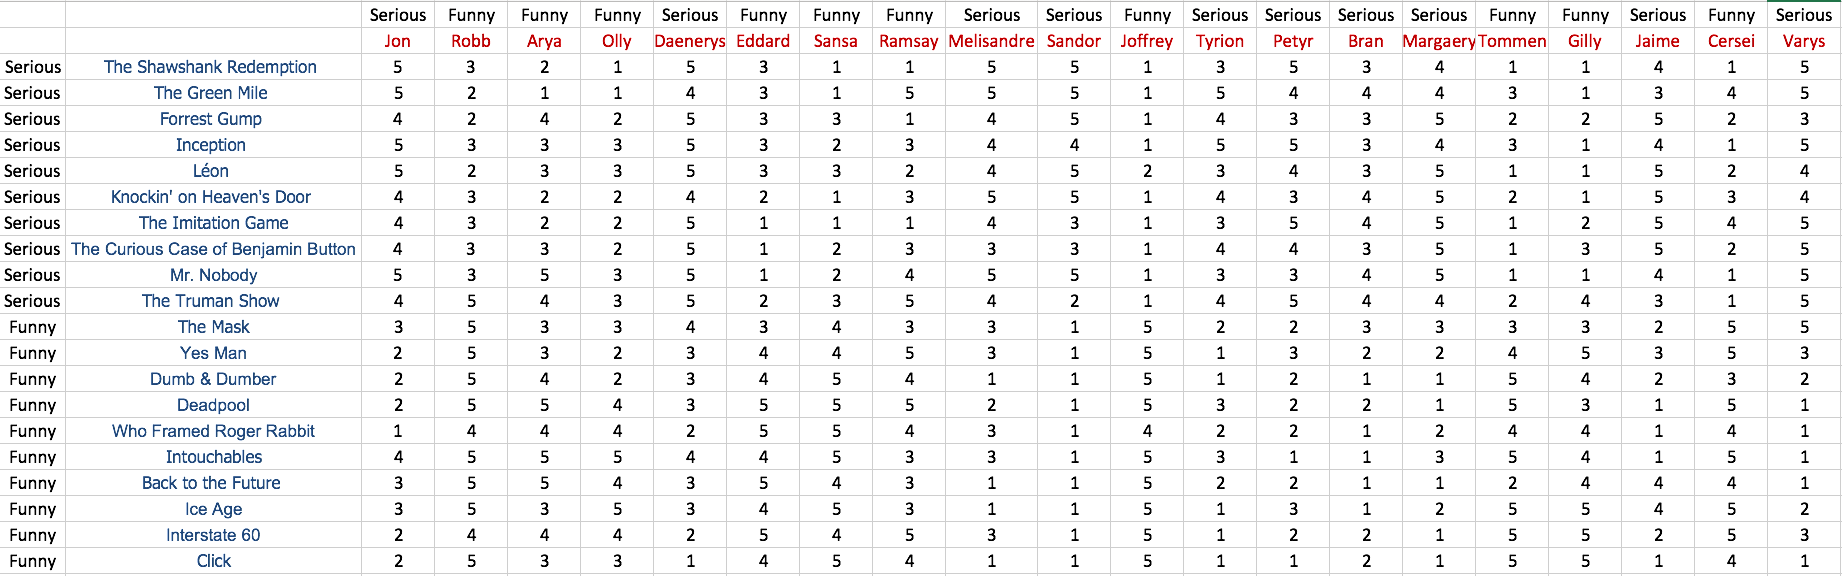
\includegraphics[width=\columnwidth]{buff1/data}
		\caption{The toy data we hand crafted. Movies and users are chacterized as funny or serious. The ratings are given accordingly with a slight noise. This is the input data used to generate plots [2-3].}
		\label{1}		
	\end{figure}
				
%	\begin{figure}[H]
%		\centering		
%		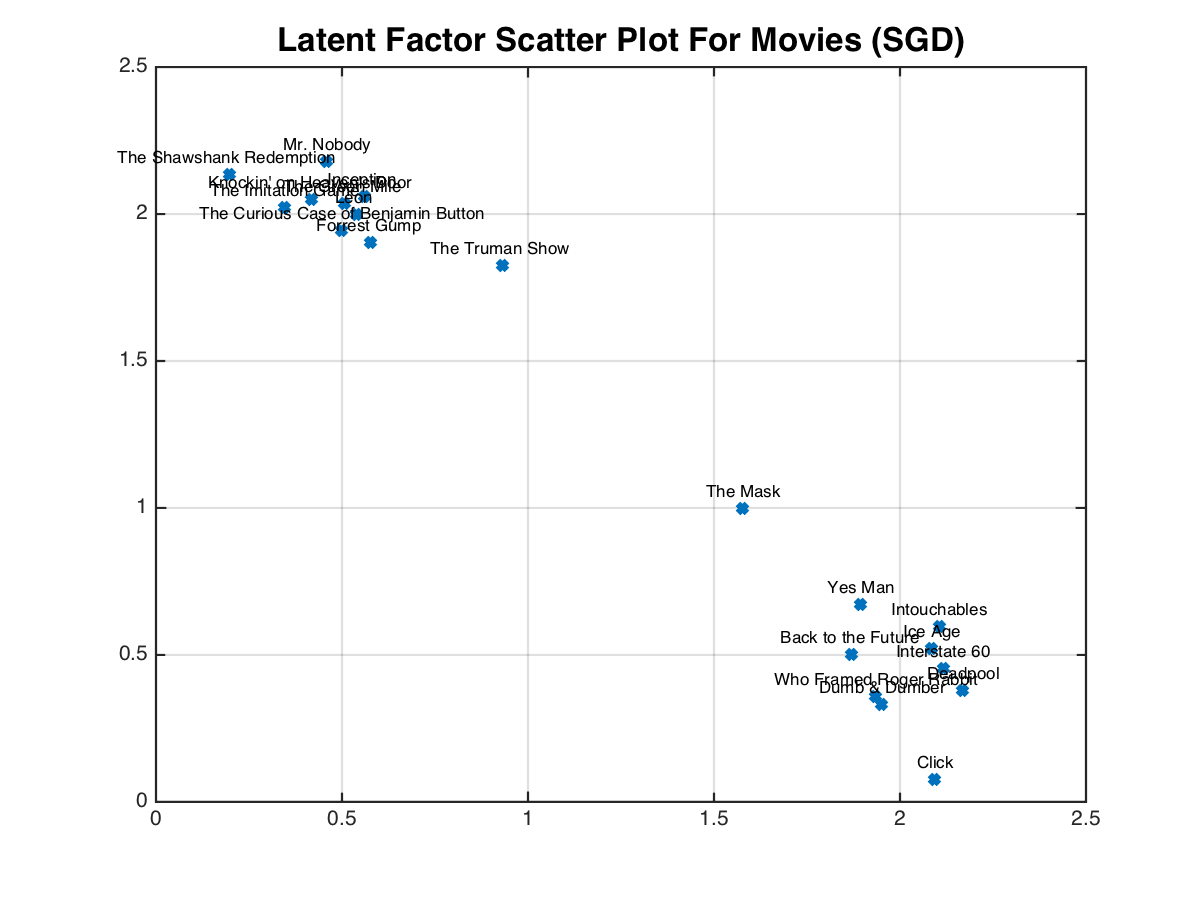
\includegraphics[width=\wi]{buff1/1}
%		\caption{Toy data clustring illustration. No missing entries in the rating matrix. Number of latent factors is 2. Trained with SGD, used plain model. This is the latent factor values for all movies. Two clusters are present as expected.}
%		\label{2}		
%	\end{figure}
%	
%	\begin{figure}[H]
%		\centering		
%		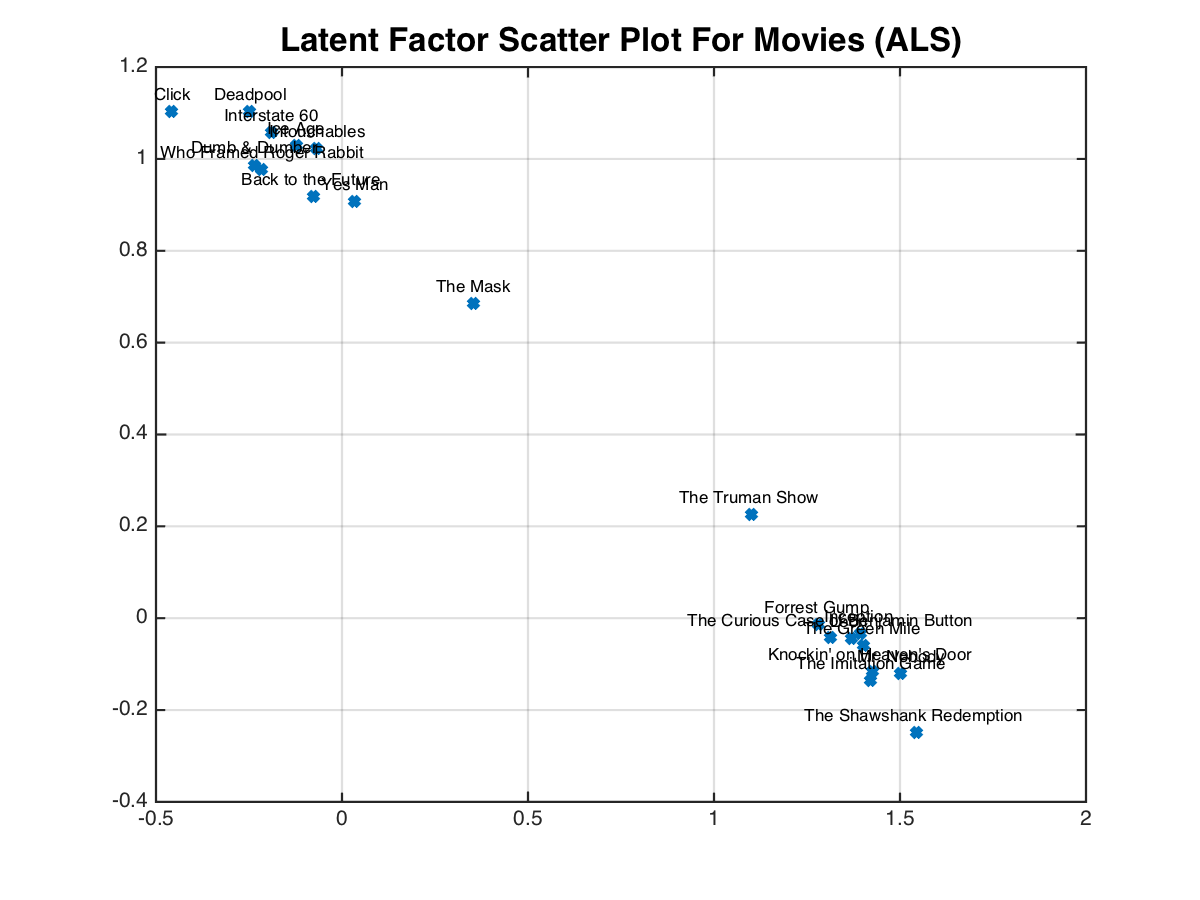
\includegraphics[width=\wi]{buff1/2}
%		\caption{Toy data clustering illustration. No missing entries in the rating matrix. Number of latent factors is 2. Trained with ALS, used plain model. This is the latent factor values for all movies. Two clusters are present as expected.}
%		\label{3}		
%	\end{figure}
	
	\begin{figure}[H]
		\centering		
		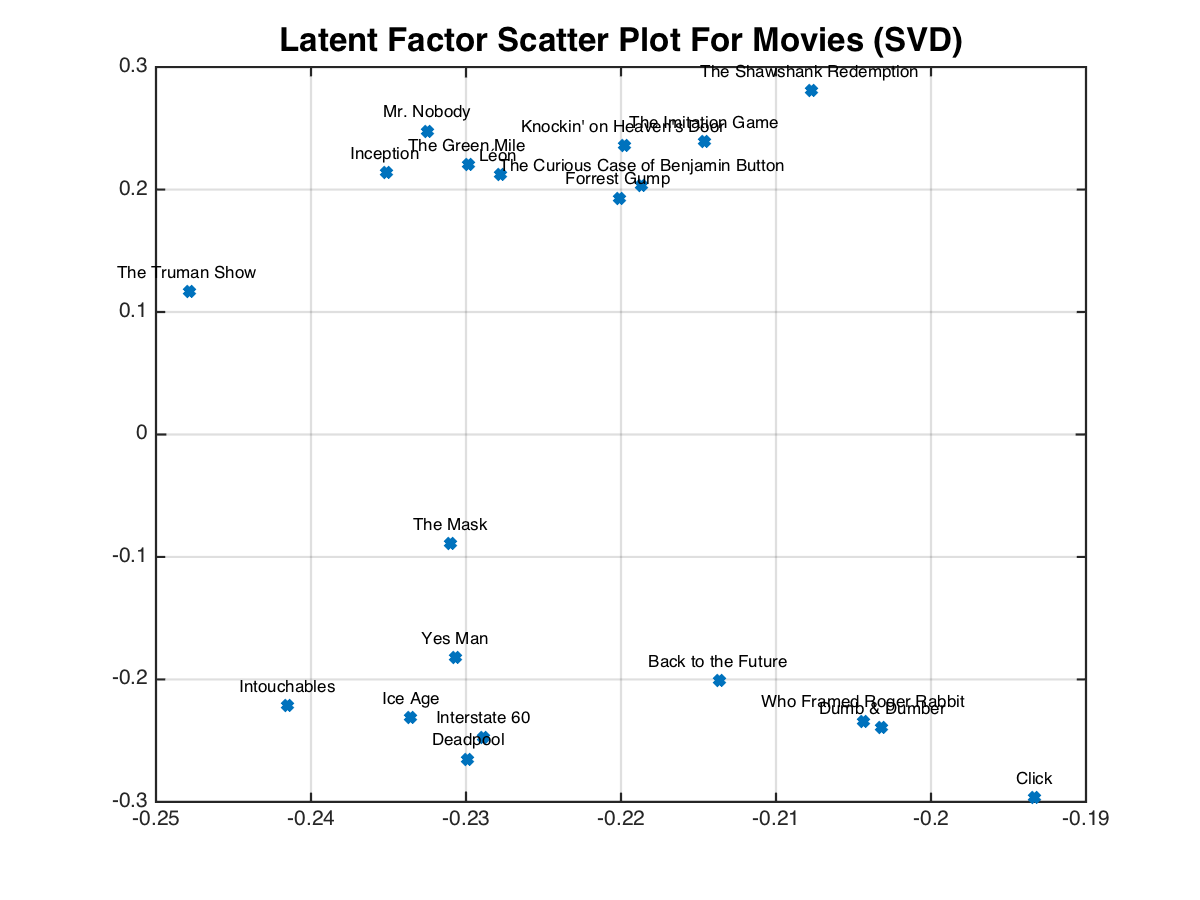
\includegraphics[width=\wi]{buff1/svd_mov}
		\caption{Toy data clustering illustration. No missing entries in the rating matrix. Number of latent factors is 2. Solved with SVD. This is the latent factor values for all movies. Two clusters are present as expected.}
		\label{4}		
	\end{figure}
	
%	\begin{figure}[H]
%		\centering		
%		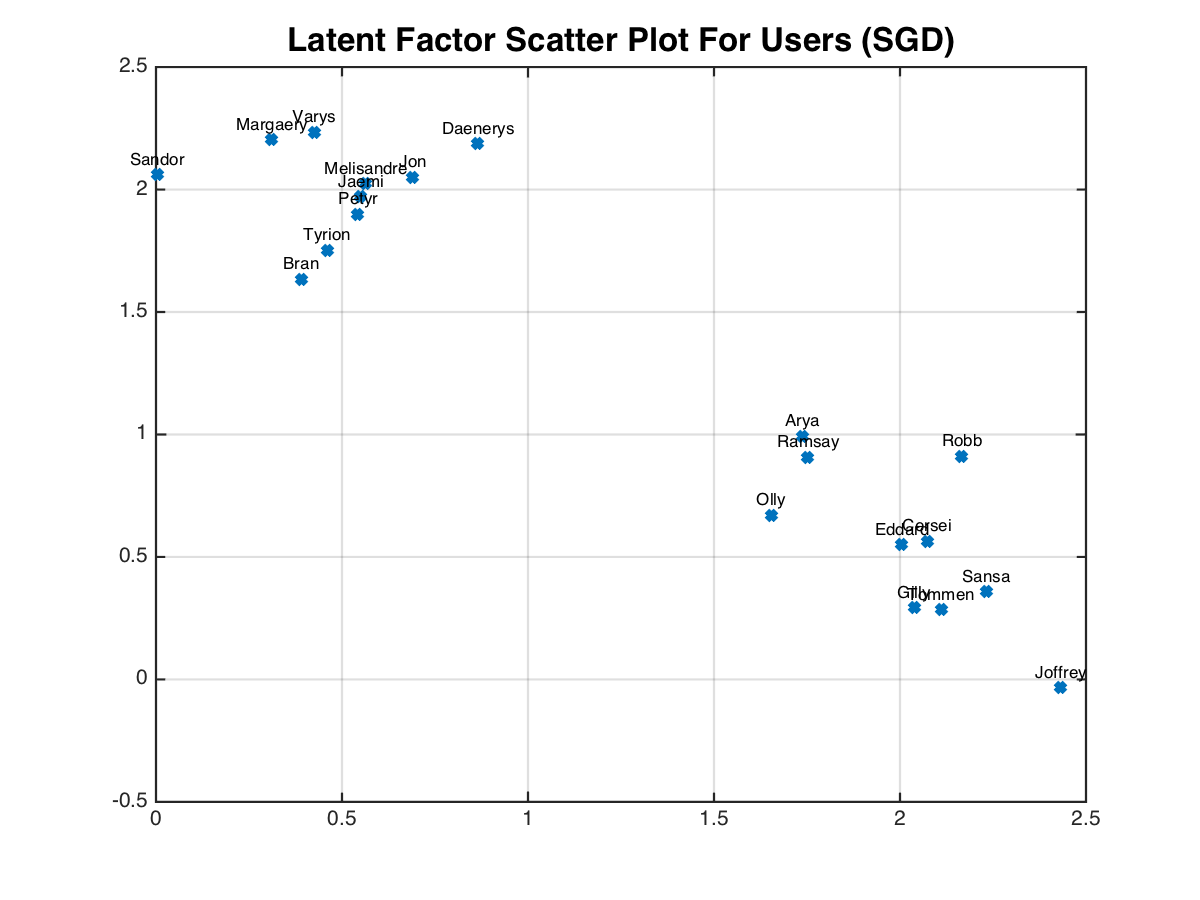
\includegraphics[width=\wi]{buff1/3}
%		\caption{Toy data clustering illustration. No missing entries in the rating matrix. Number of latent factors is 2. Trained with SGD, used plain model. This is the latent factor values for all users. Two clusters are present as expected.}
%		\label{5}		
%	\end{figure}
%							
%	\begin{figure}[H]
%		\centering		
%		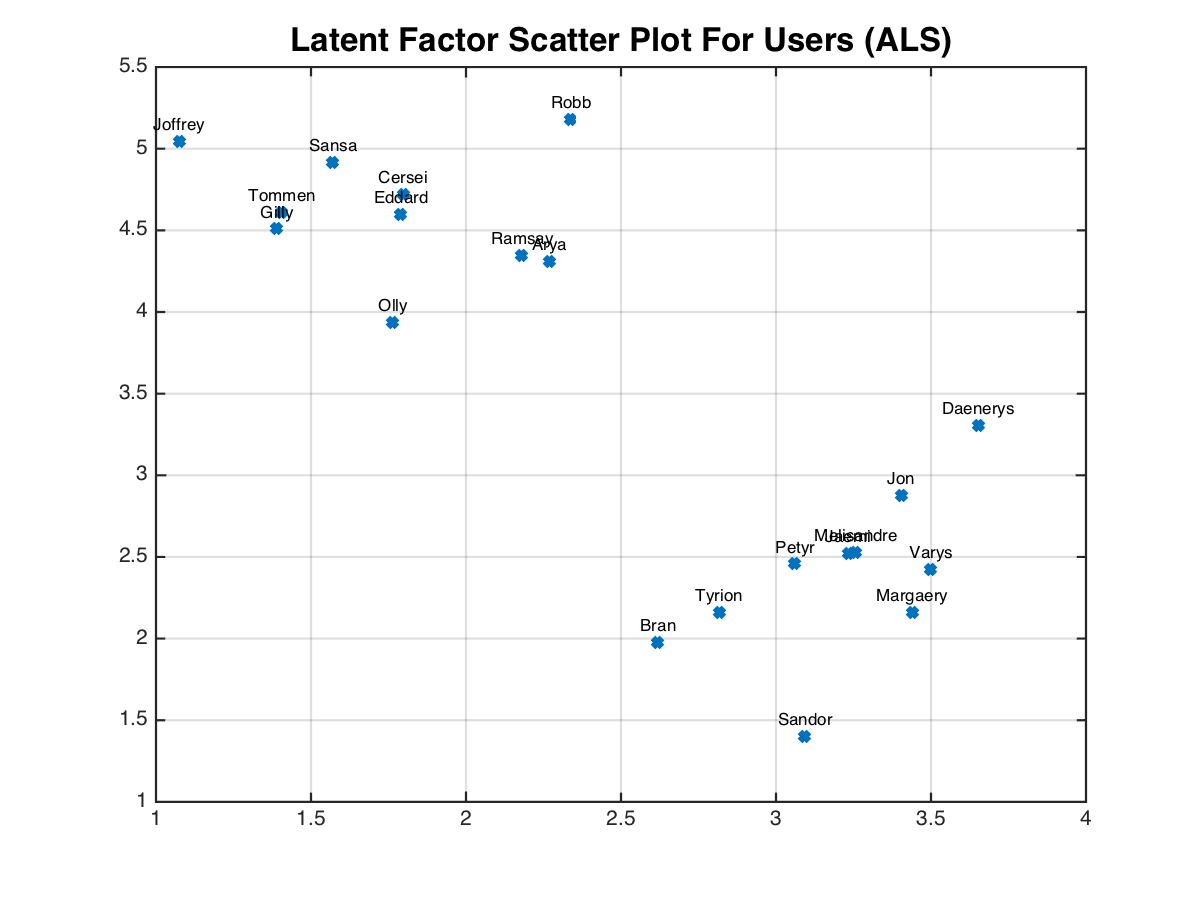
\includegraphics[width=\wi]{buff1/4}
%		\caption{Toy data clustering illustration. No missing entries in the rating matrix. Number of latent factors is 2. Trained with ALS, used plain model. This is the latent factor values for all users. Two clusters are present as expected.}
%		\label{6}		
%	\end{figure}
	
	\begin{figure}[H]
		\centering		
		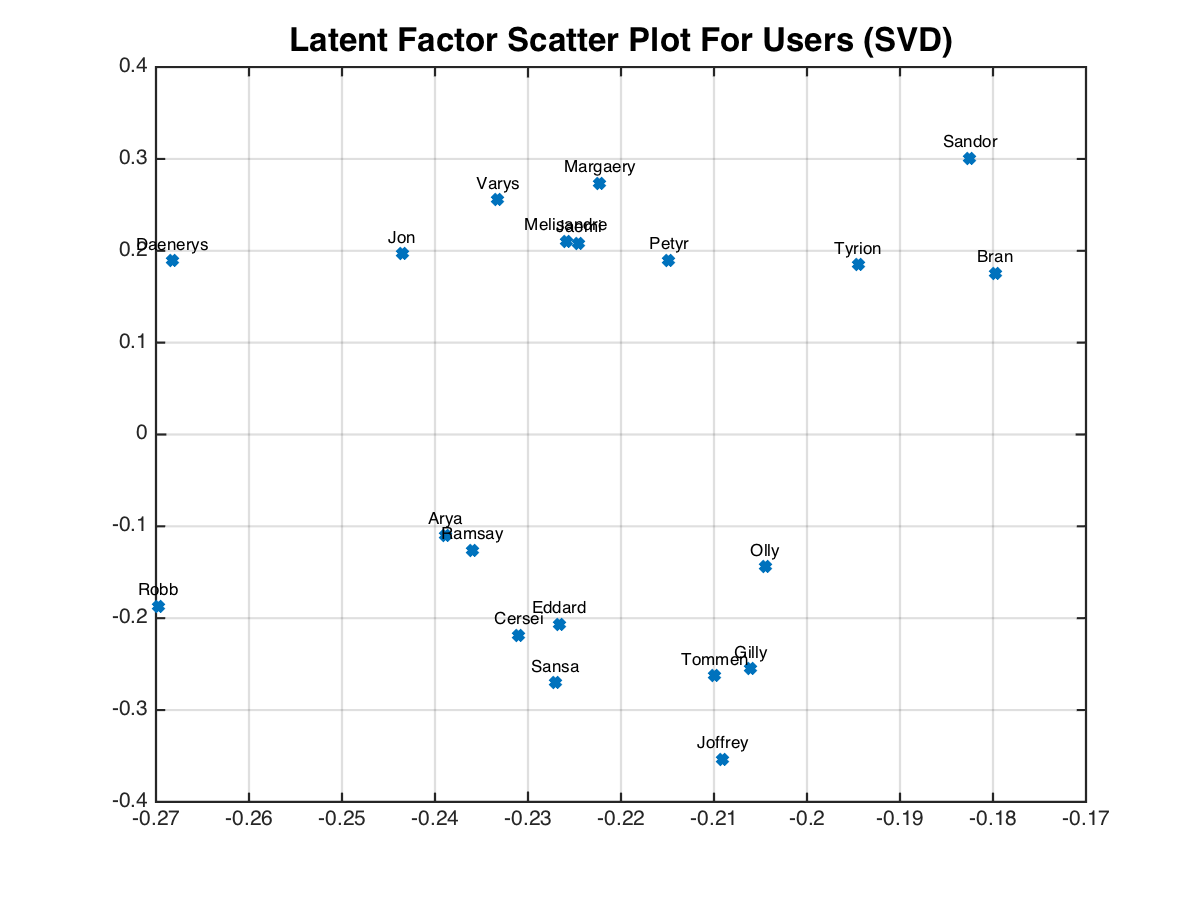
\includegraphics[width=\wi]{buff1/svd_user}
		\caption{Toy data clustering illustration. No missing entries in the rating matrix. Number of latent factors is 2. Solved with SVD. This is the latent factor values for all users. Two clusters are present as expected.}
		\label{7}		
	\end{figure}
	
%	\begin{figure}[H]
%		\centering		
%		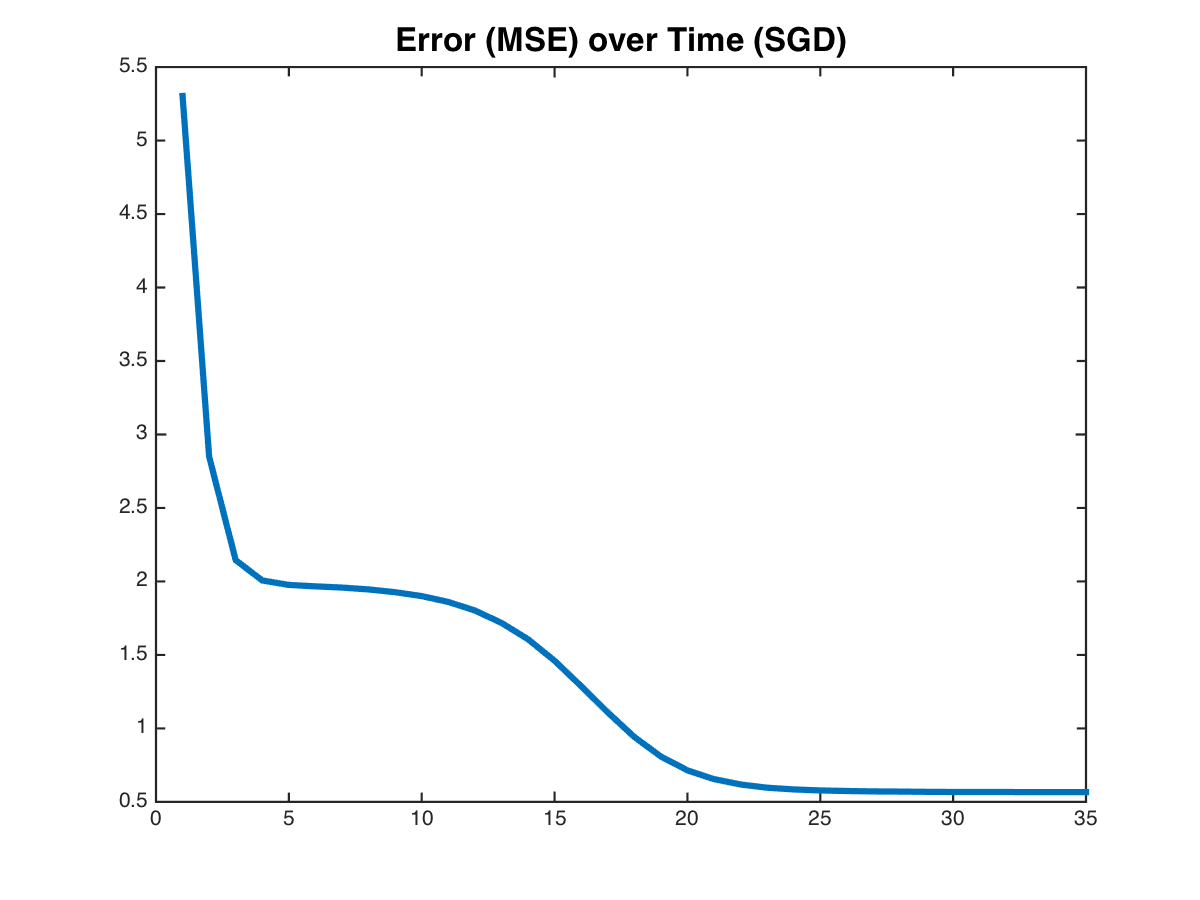
\includegraphics[width=\wiq]{buff1/5}
%		\caption{Toy data illustration. No missing entries in the rating matrix. Plot of mean square error versus epoch using SGD. Where epoch is one iteration through whole dataset. Notice that a larger learning rate might have cause an oscillation at the error level of 2. Time elapsed: 0.1093 sec}
%		\label{8}		
%	\end{figure}
%	\begin{figure}[H]
%		\centering		
%		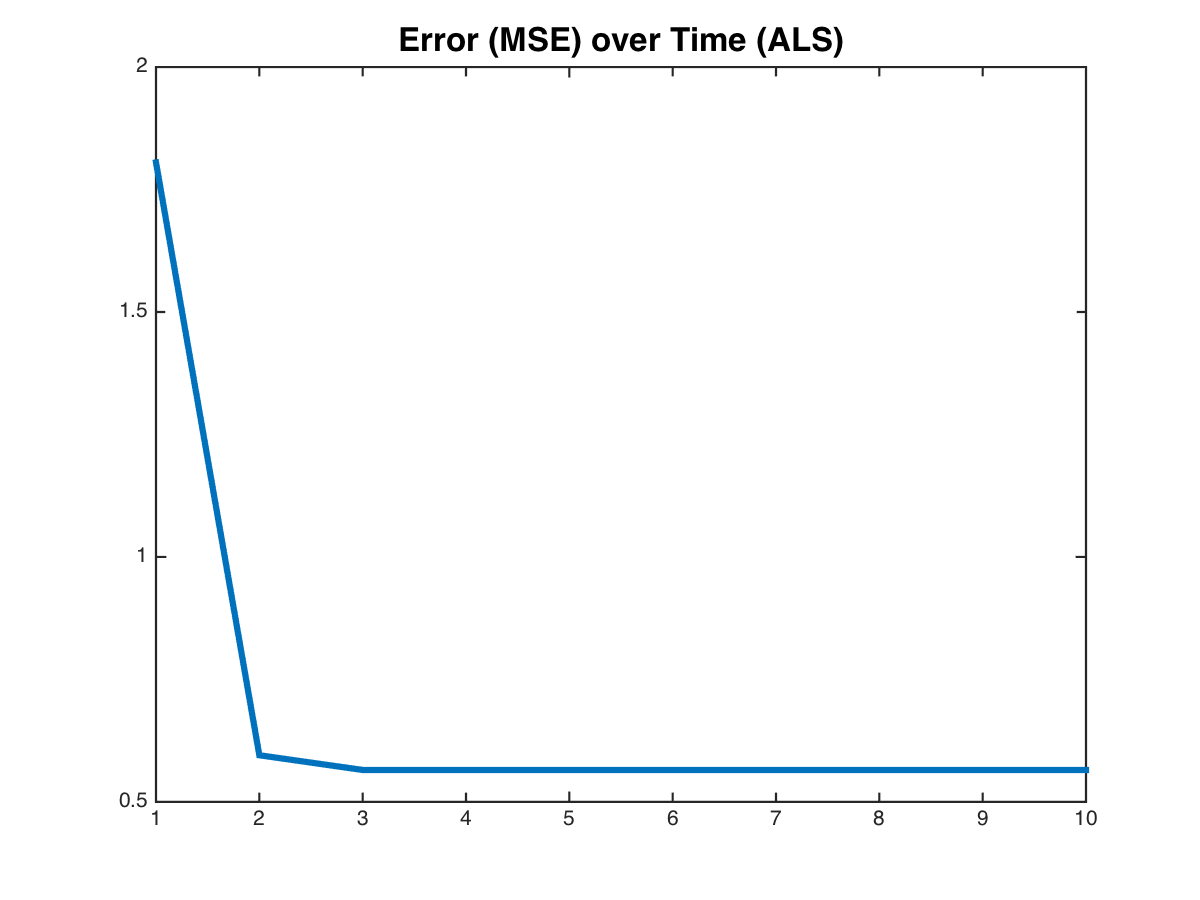
\includegraphics[width=\wi]{buff1/6}
%		\caption{Toy data illustration. No missing entries in the rating matrix. Plot of mean square error versus iteration. One iteration is defined as solving least squares once both for $U$ and $I_T$. Time elapsed: 0.0525 sec. Converges faster than SGD. As expected, ALS has good performance when the data is not sparse.}
%		\label{9}		
%	\end{figure}
				
	
	\clearpage
	\begin{figure}[H]
		\centering		
		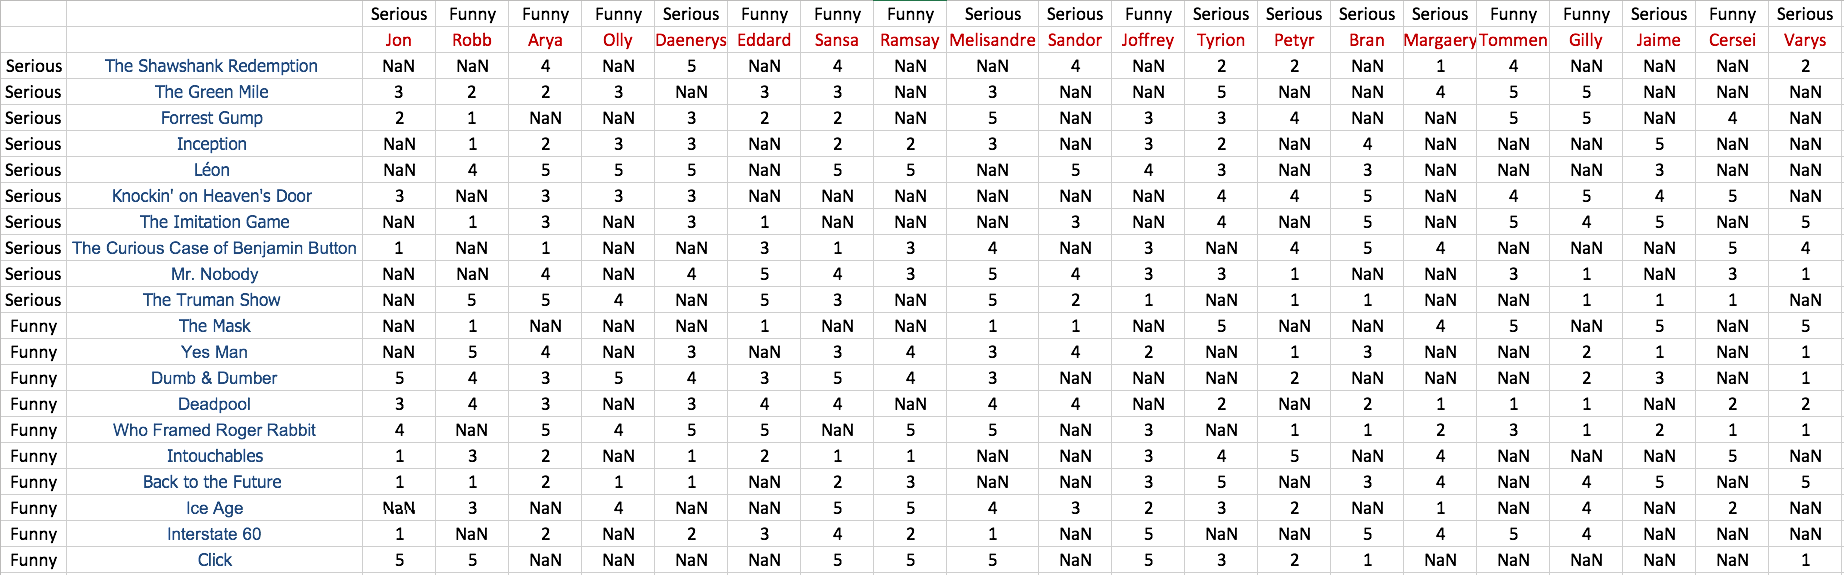
\includegraphics[width=\columnwidth]{buff2/data}
		\caption{The toy data we hand crafted. Movies and users are chacterized as funny or serious. The ratings are given accordingly with a slight noise. Some entries are hidden. This is the input data used to generate plots [5-18].}
		\label{5}		
	\end{figure}
	
	\begin{figure}[H]
		\centering		
		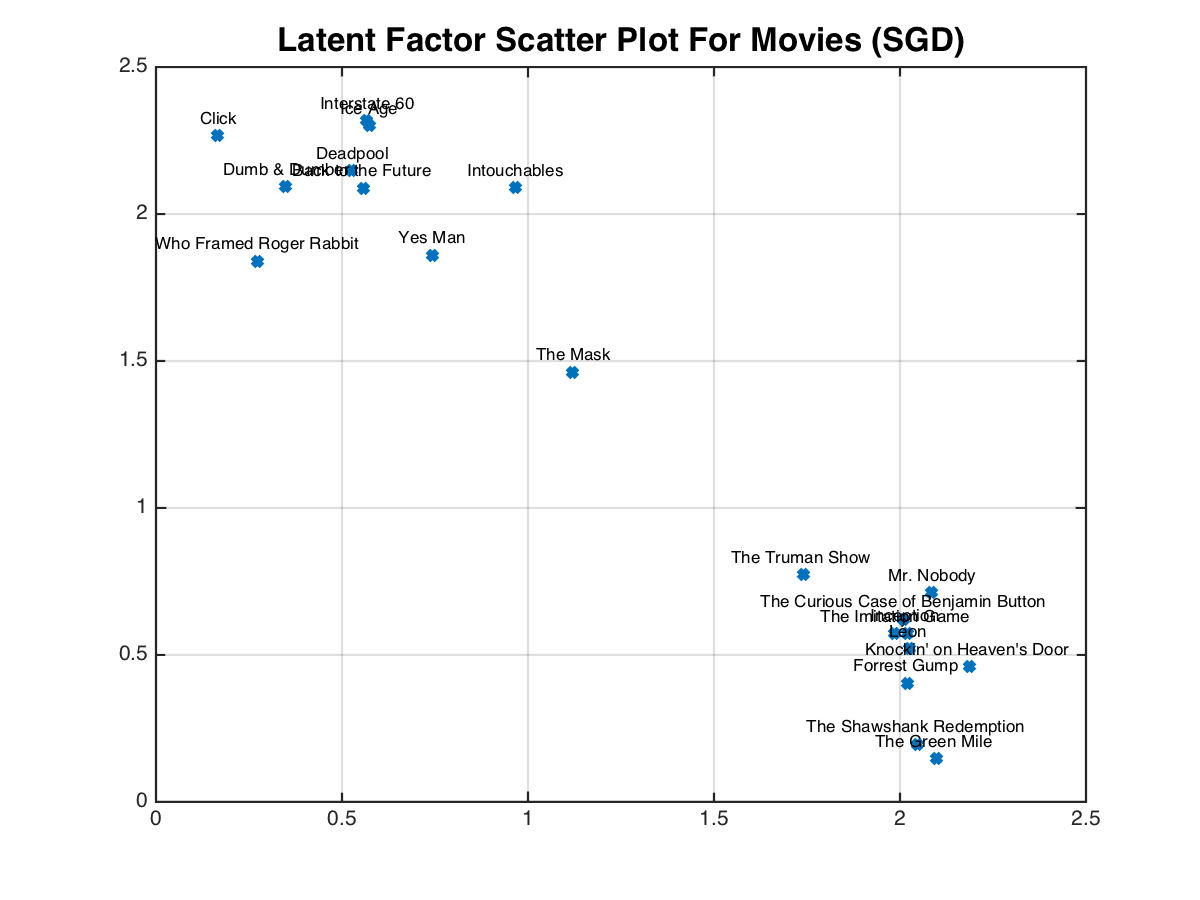
\includegraphics[width=\columnwidth]{buff2/1}
		\caption{Toy data clustring illustration. Half of the entries are missing in the rating matrix. Number of latent factors is 2. Trained with SGD, used plain model. This is the latent factor values for all movies. Two clusters are present as expected. The amount of data is enough to spot the patterns.}
		\label{5}		
	\end{figure}
	\begin{figure}[H]
		\centering		
		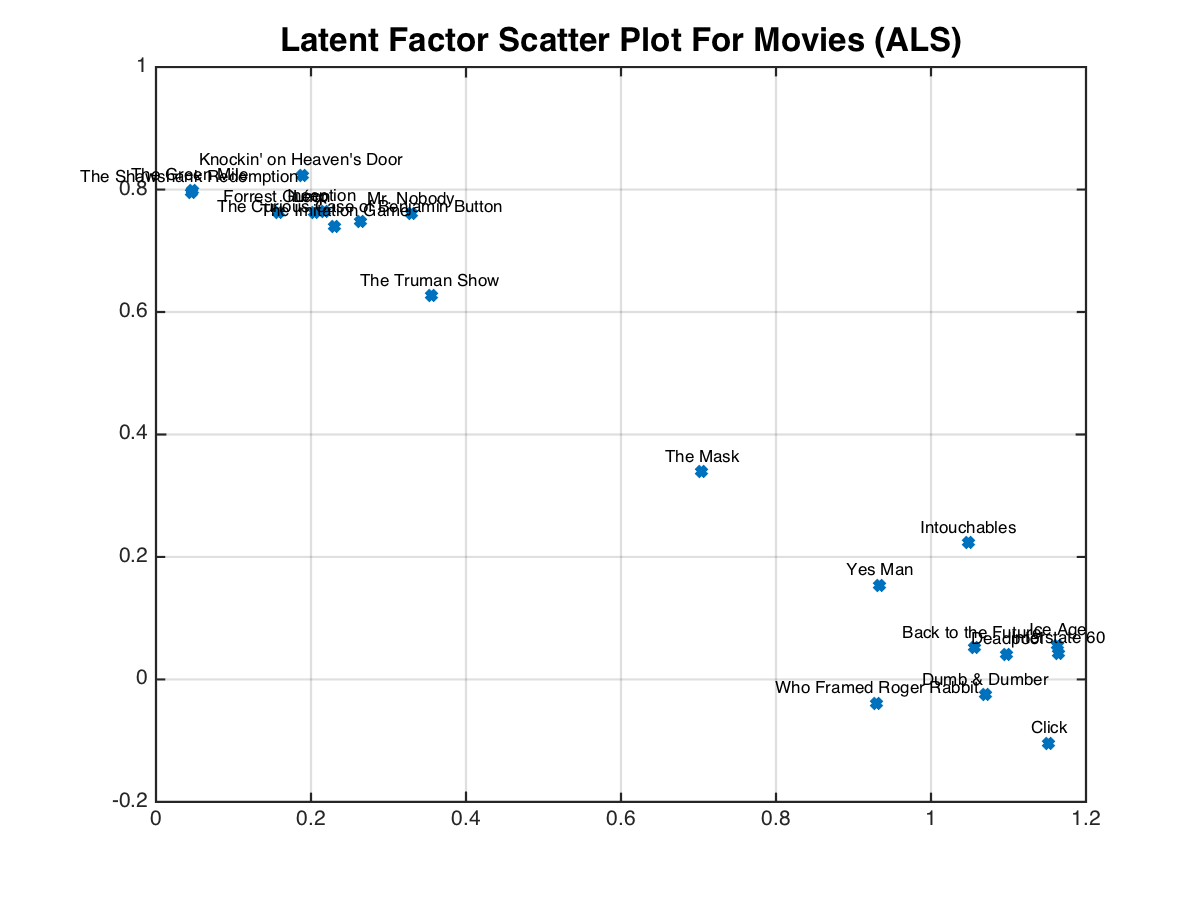
\includegraphics[width=\wiq]{buff2/2}
		\caption{Toy data clustring illustration. Half of the entries are missing in the rating matrix. Number of latent factors is 2. Trained with ALS, used plain model. This is the latent factor values for all movies. Two clusters are present as expected. The amount of data is enough to spot the patterns. Notice that we cannot call Matlab's \textbf{svd()} because there are missing entries.}
		\label{5}		
	\end{figure}
	\begin{figure}[H]
		\centering		
		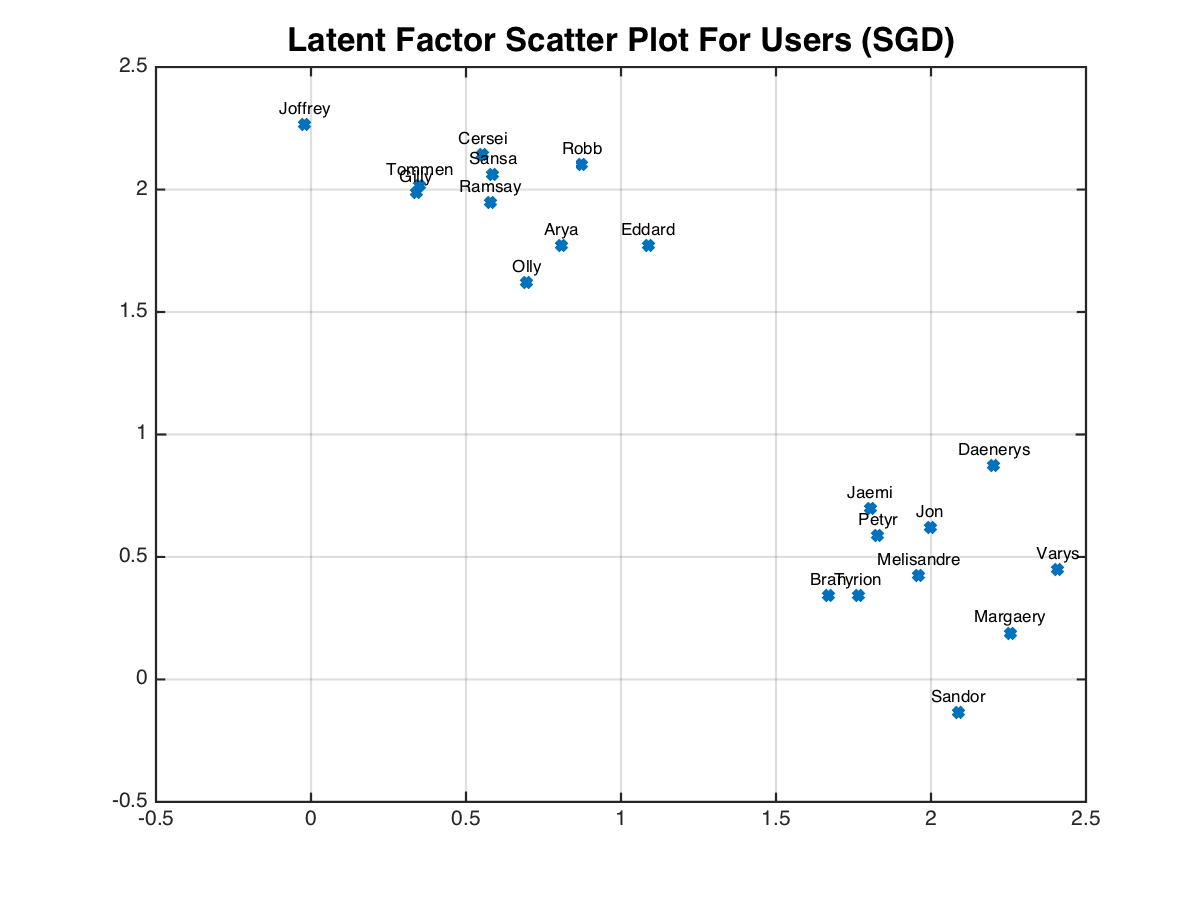
\includegraphics[width=\wi]{buff2/3}
		\caption{Toy data clustring illustration. Half of the entries are missing in the rating matrix. Number of latent factors is 2. Trained with SGD, used plain model. This is the latent factor values for all users. Two clusters are present as expected. The amount of data is enough to spot the patterns.}
		\label{5}		
	\end{figure}						
	\begin{figure}[H]
		\centering		
		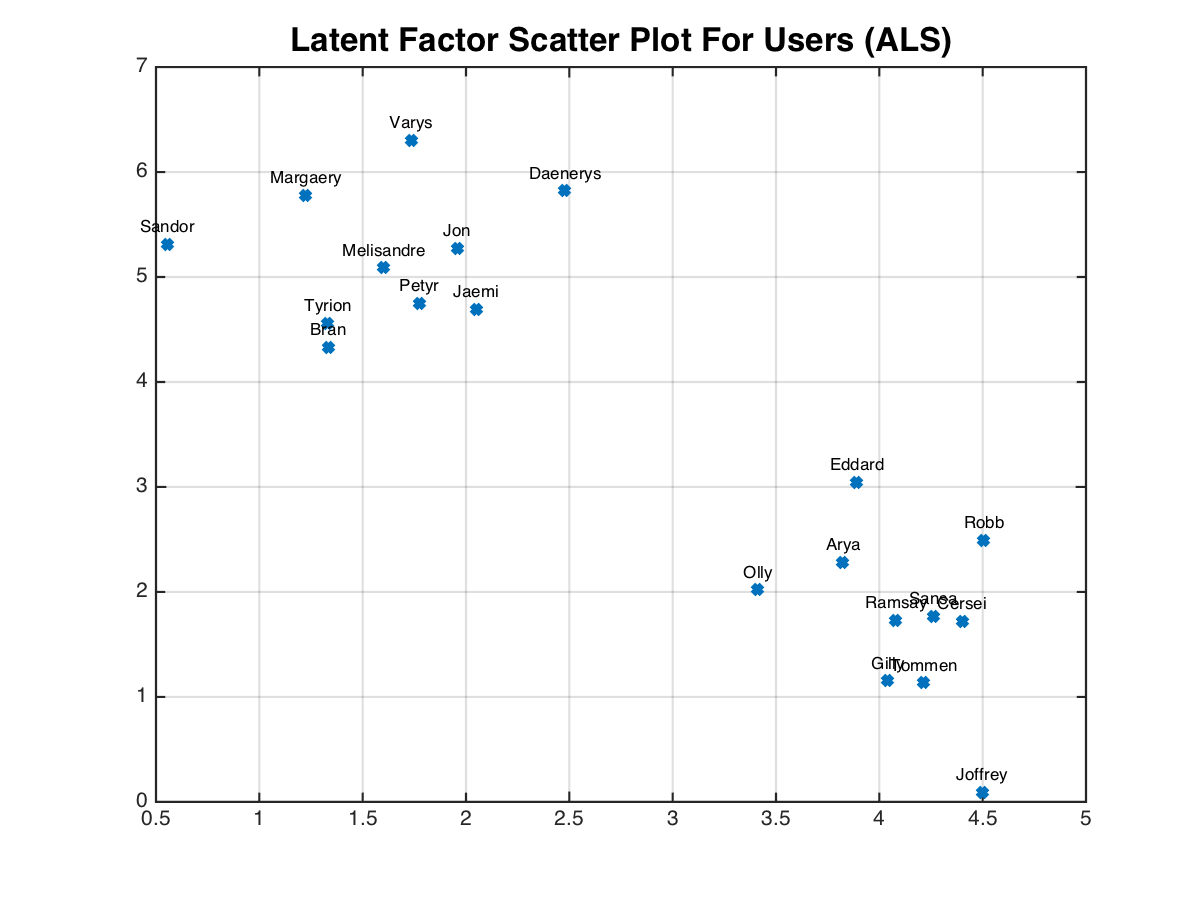
\includegraphics[width=\wiq]{buff2/4}
		\caption{Toy data clustring illustration. Half of the entries are missing in the rating matrix. Number of latent factors is 2. Trained with ALS, used plain model. This is the latent factor values for all users. Two clusters are present as expected. The amount of data is enough to spot the patterns.}
		\label{5}		
	\end{figure}						
	\begin{figure}[H]
		\centering		
		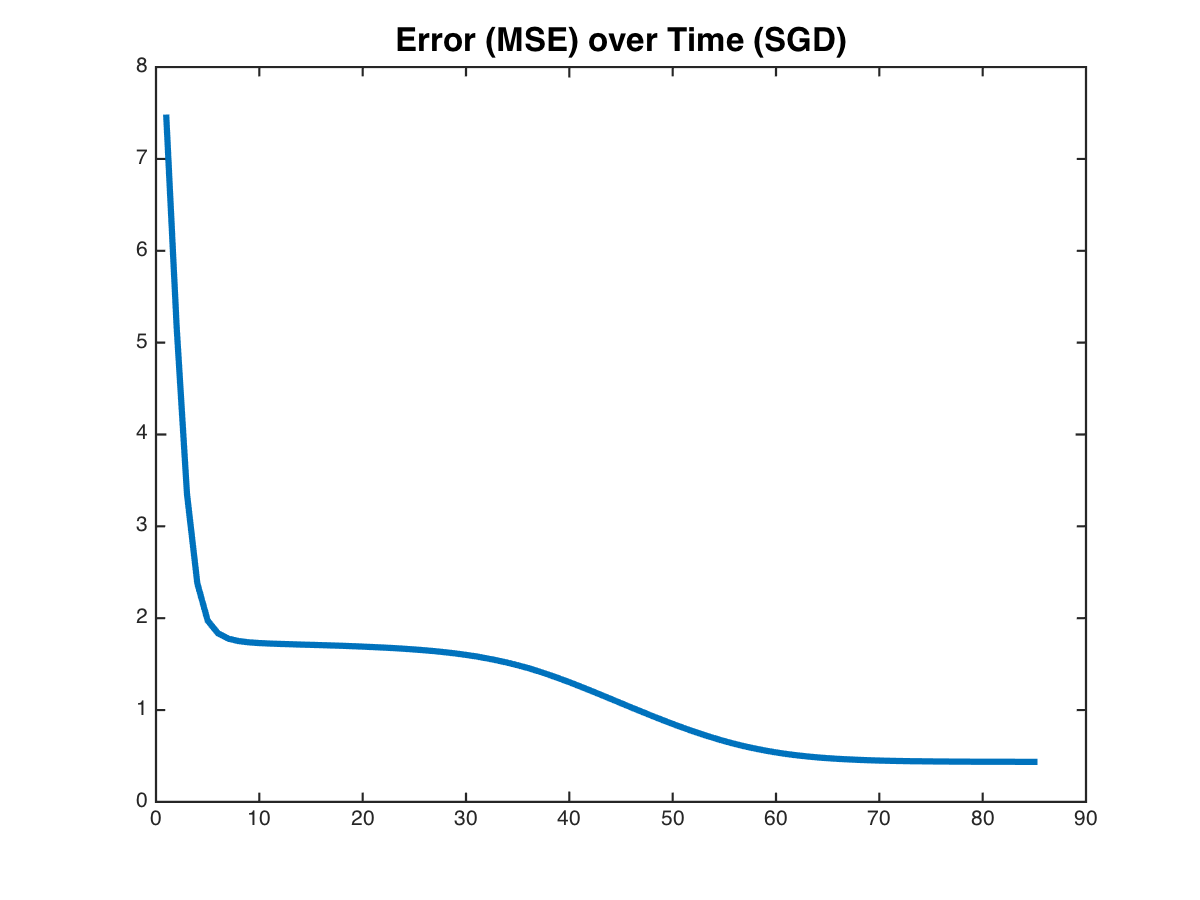
\includegraphics[width=\wi]{buff2/5}
		\caption{Toy data illustration. Half of the entries are missing in the rating matrix. Plot of mean square error versus epoch using SGD. Where epoch is one iteration through whole dataset. Notice that a larger learning rate might have cause an oscillation at the error level of 2. Time elapsed: 0.1603 sec}
		\label{5}		
	\end{figure}
	\begin{figure}[H]
		\centering		
		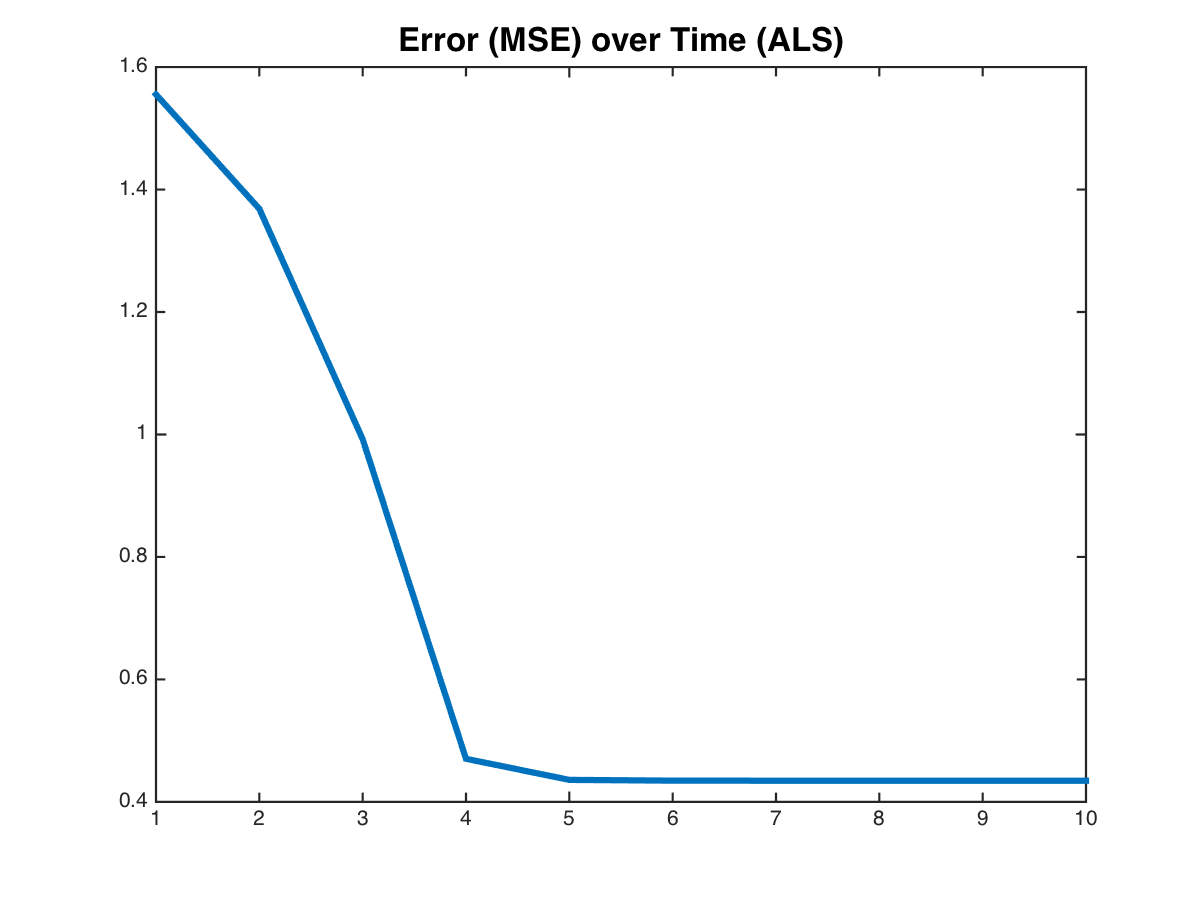
\includegraphics[width=\wi]{buff2/6}
		\caption{Toy data illustration. Half of the entries are missing in the rating matrix. Plot of mean square error versus iteration. One iteration is defined as solving least squares once both for $U$ and $I_T$. Time elapsed: 0.0313 sec. Converges faster than SGD. As expected, ALS has good performance when the data is not sparse.}
		\label{5}		
	\end{figure}
	
	
	
	
	\begin{figure}[H]
		\centering		
		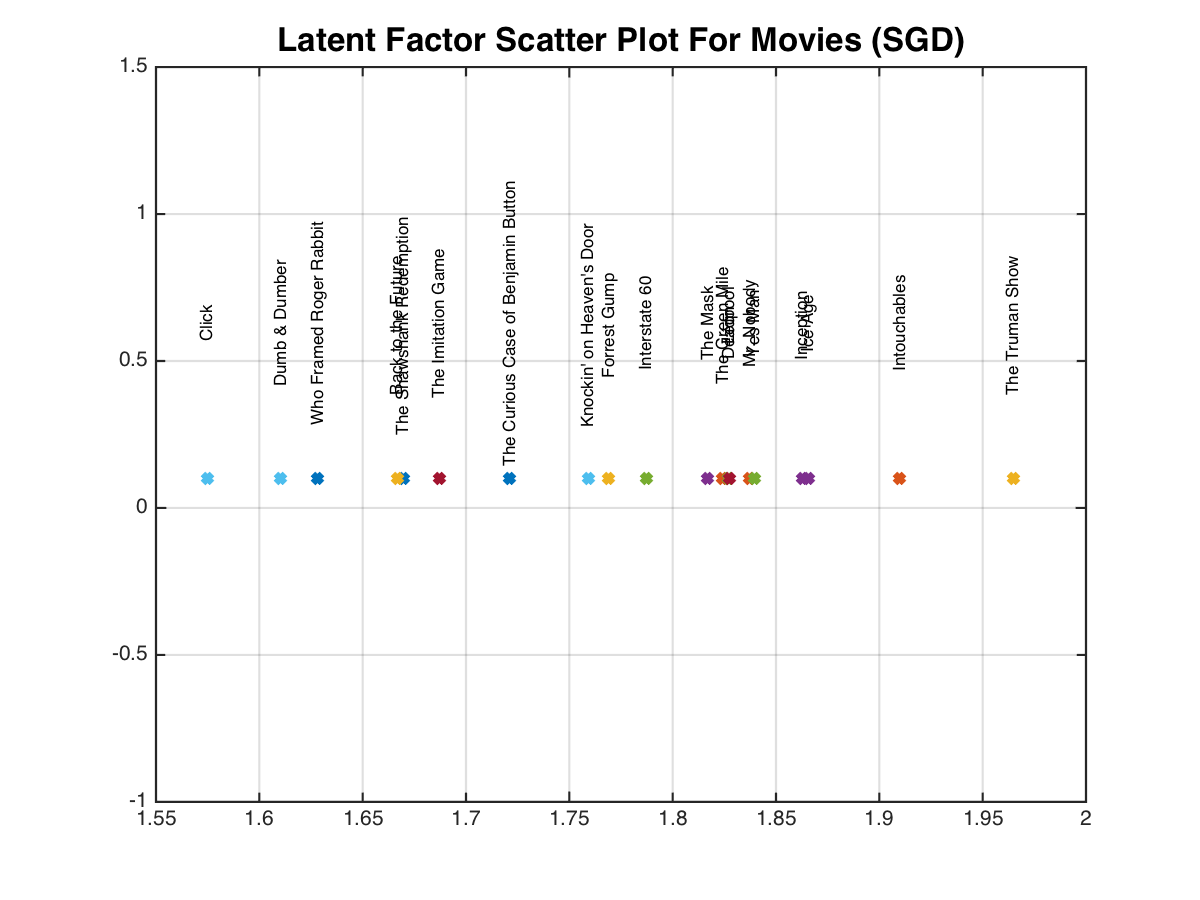
\includegraphics[width=\wiq]{buff3/1}
		\caption{Toy data clustring illustration. Half of the entries are missing in the rating matrix. Number of latent factors is 1. Trained with SGD, used plain model. This is the latent factor values for all movies. No clusters can be spotted in spite of the case where number of latent factors were two. This points out that one factor is too small to capture the characteristics.}
		\label{5}		
	\end{figure}
	\begin{figure}[H]
		\centering		
		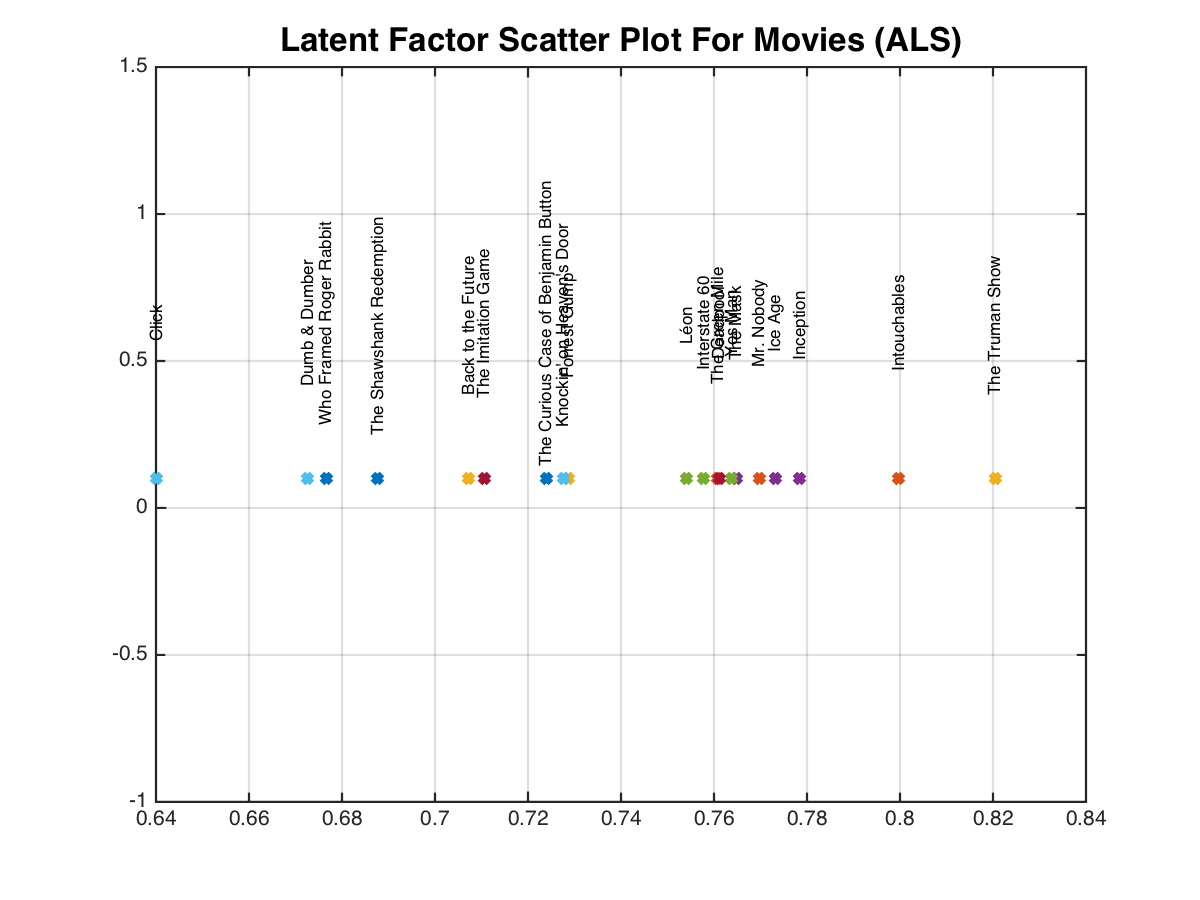
\includegraphics[width=\wiq]{buff3/2}
		\caption{Toy data clustring illustration. Half of the entries are missing in the rating matrix. Number of latent factors is 1. Trained with ALS, used plain model. This is the latent factor values for all movies. No clusters can be spotted in spite of the case where number of latent factors were two. This points out that one factor is too small to capture the characteristics.}
		\label{5}		
	\end{figure}

	\begin{figure}[H]
		\centering		
		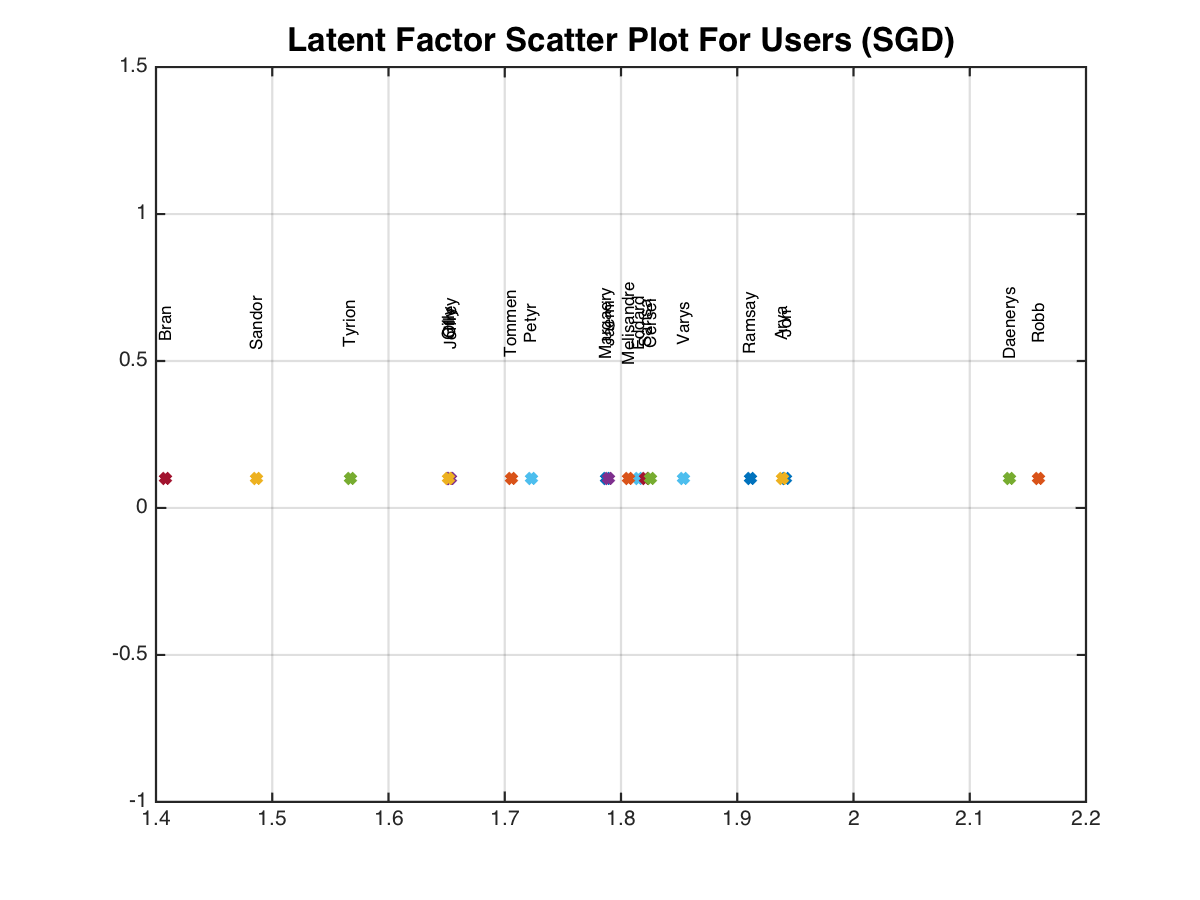
\includegraphics[width=\wi]{buff3/3}
		\caption{Toy data clustring illustration. Half of the entries are missing in the rating matrix. Number of latent factors is 1. Trained with SGD, used plain model. This is the latent factor values for all users. No clusters can be spotted in spite of the case where number of latent factors were two. This points out that one factor is too small to capture the characteristics.}
		\label{5}		
	\end{figure}						
	\begin{figure}[H]
		\centering		
		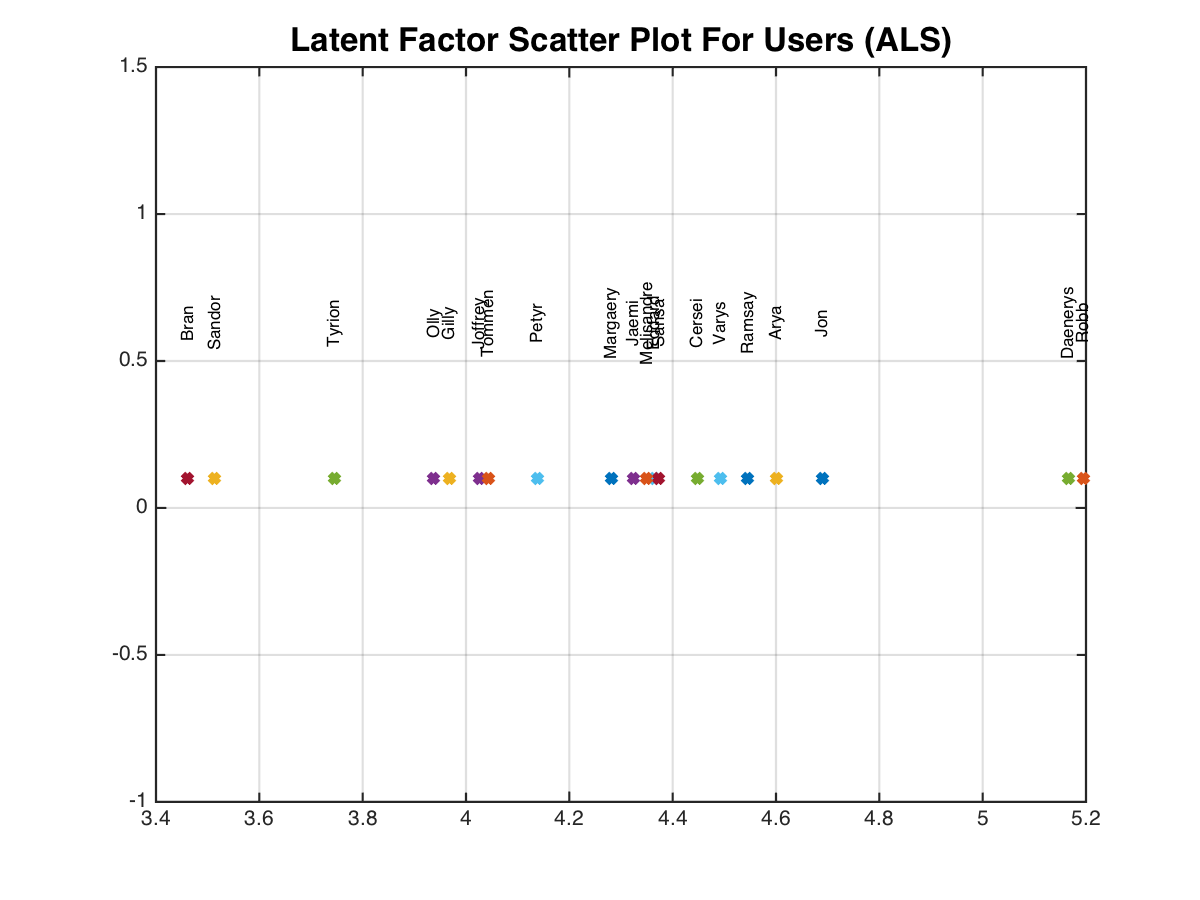
\includegraphics[width=\wi]{buff3/4}
		\caption{Toy data clustring illustration. Half of the entries are missing in the rating matrix. Number of latent factors is 1. Trained with ALS, used plain model. This is the latent factor values for all movies. No clusters can be spotted in spite of the case where number of latent factors were two. This points out that one factor is too small to capture the characteristics.}
		\label{5}		
	\end{figure}
	\begin{figure}[H]
		\centering		
		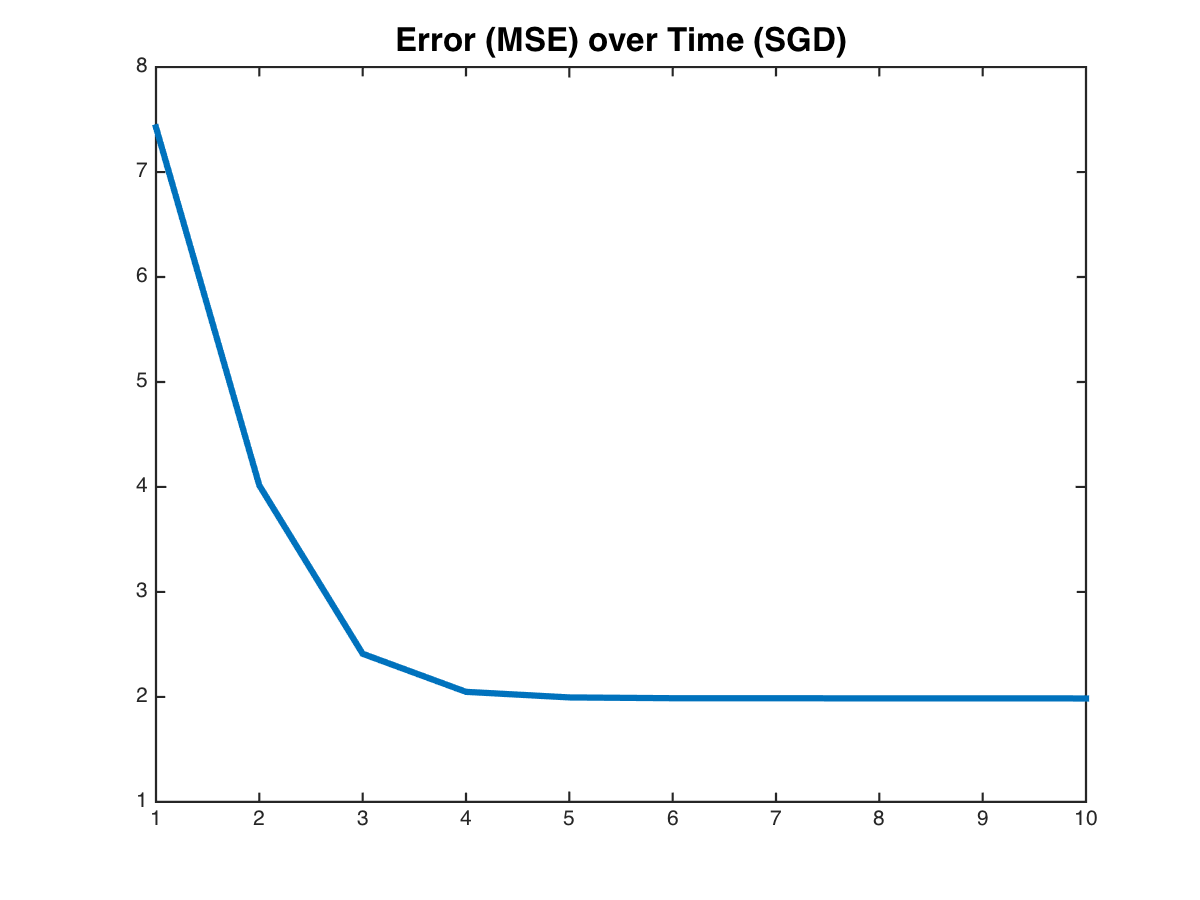
\includegraphics[width=\wi]{buff3/5}
		\caption{Toy data illustration. Half of the entries are missing in the rating matrix. Plot of mean square error versus epoch using SGD. Where epoch is one iteration through whole dataset. Time elapsed: 0.0541 sec}
		\label{5}		
	\end{figure}
	\begin{figure}[H]
		\centering		
		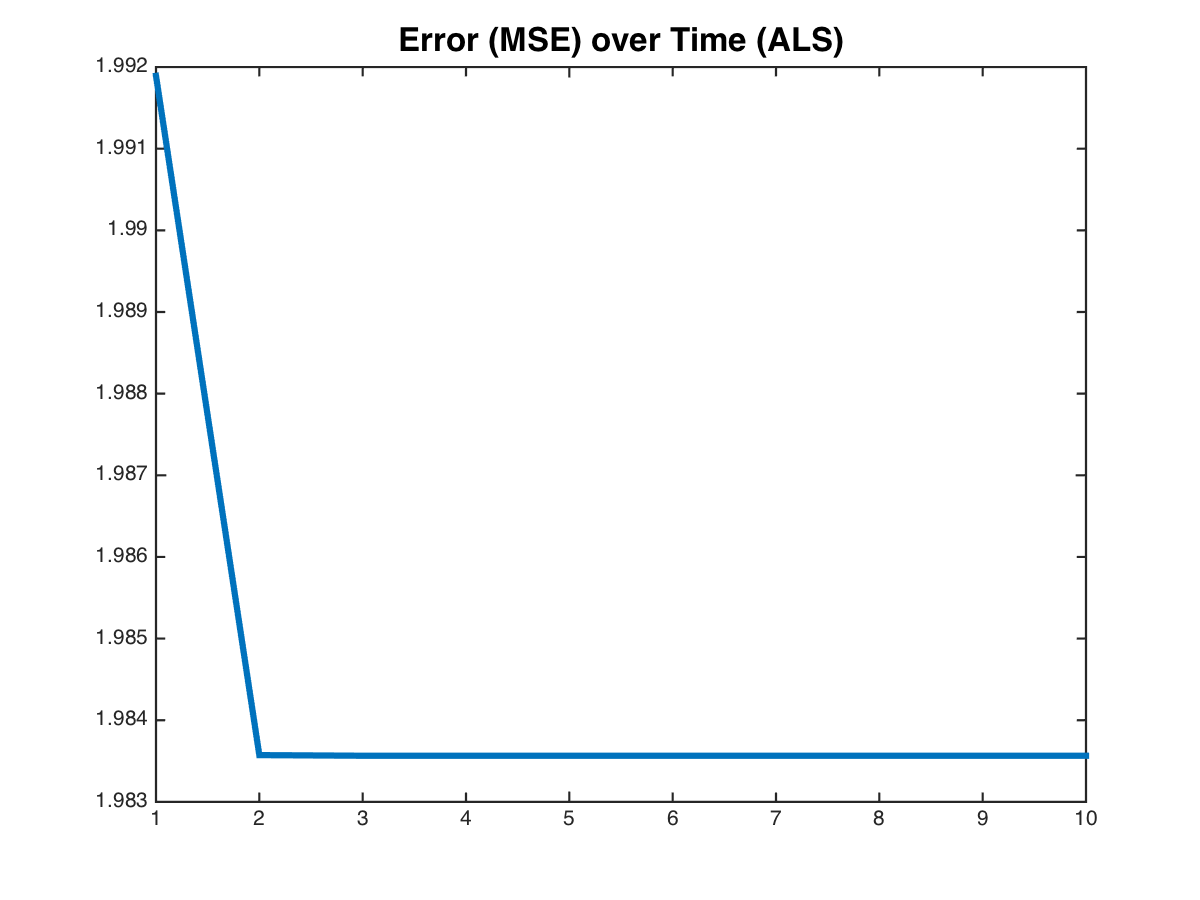
\includegraphics[width=\wi]{buff3/6}
		\caption{Toy data illustration. Half of the entries are missing in the rating matrix. Plot of mean square error versus iteration. One iteration is defined as solving least squares once both for $U$ and $I_T$. Time elapsed: 0.0408 sec. Converges faster than SGD. As expected, ALS has good performance when the data is not sparse.}
		\label{5}		
	\end{figure}
	
	
	
	
	
	\begin{figure}[H]
		\centering		
		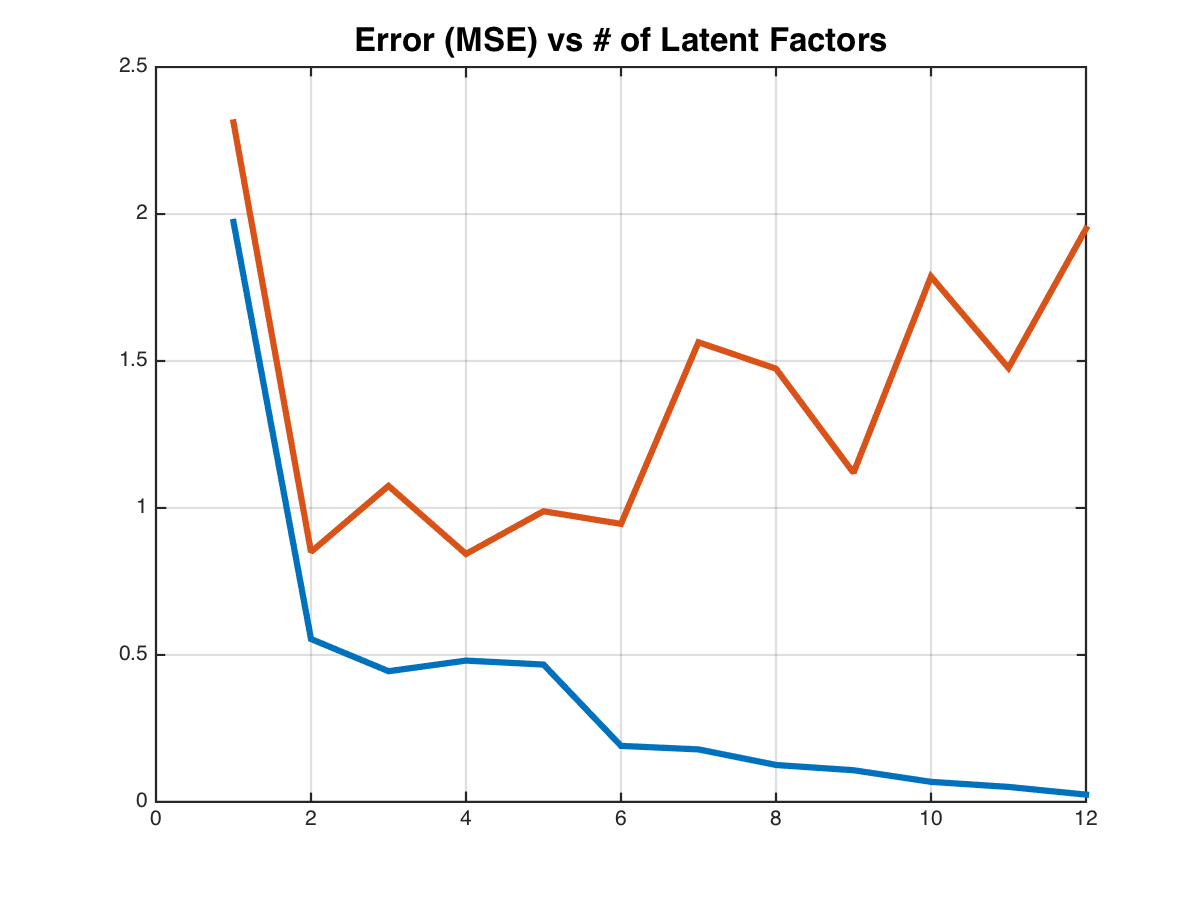
\includegraphics[width=\wi]{buff4/l_sgd_toy}
		\caption{Toy data illustration. Half of the entries are missing in the rating matrix. This plot demonstrates how error on training (blue) and test (red) data changes according to number of latent factors when the model is trained with SGD. }
		\label{5}		
	\end{figure}
	\clearpage
	
	\begin{figure}[H]
		\centering		
		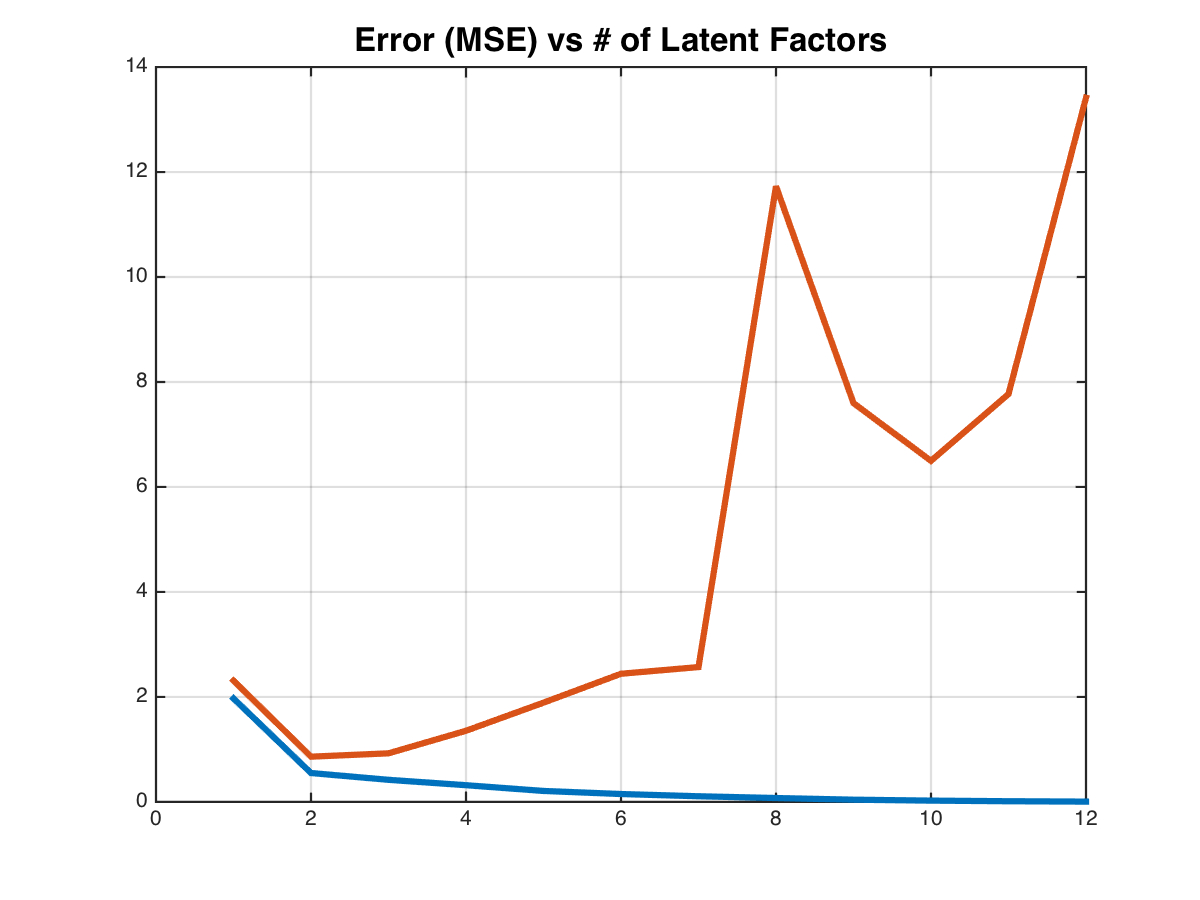
\includegraphics[width=\wi]{buff4/l_als_toy}
		\caption{Toy data illustration. Half of the entries are missing in the rating matrix. This plot demonstrates how error on training (blue) and test (red) data changes according to number of latent factors when the model is trained with ALS. }
		\label{5}		
	\end{figure}


	\begin{center}
		\Large \textbf{\underline{Tests on MovieLens Data}}
	\end{center}		
	
	
	
	\begin{figure}[H]
		\centering		
		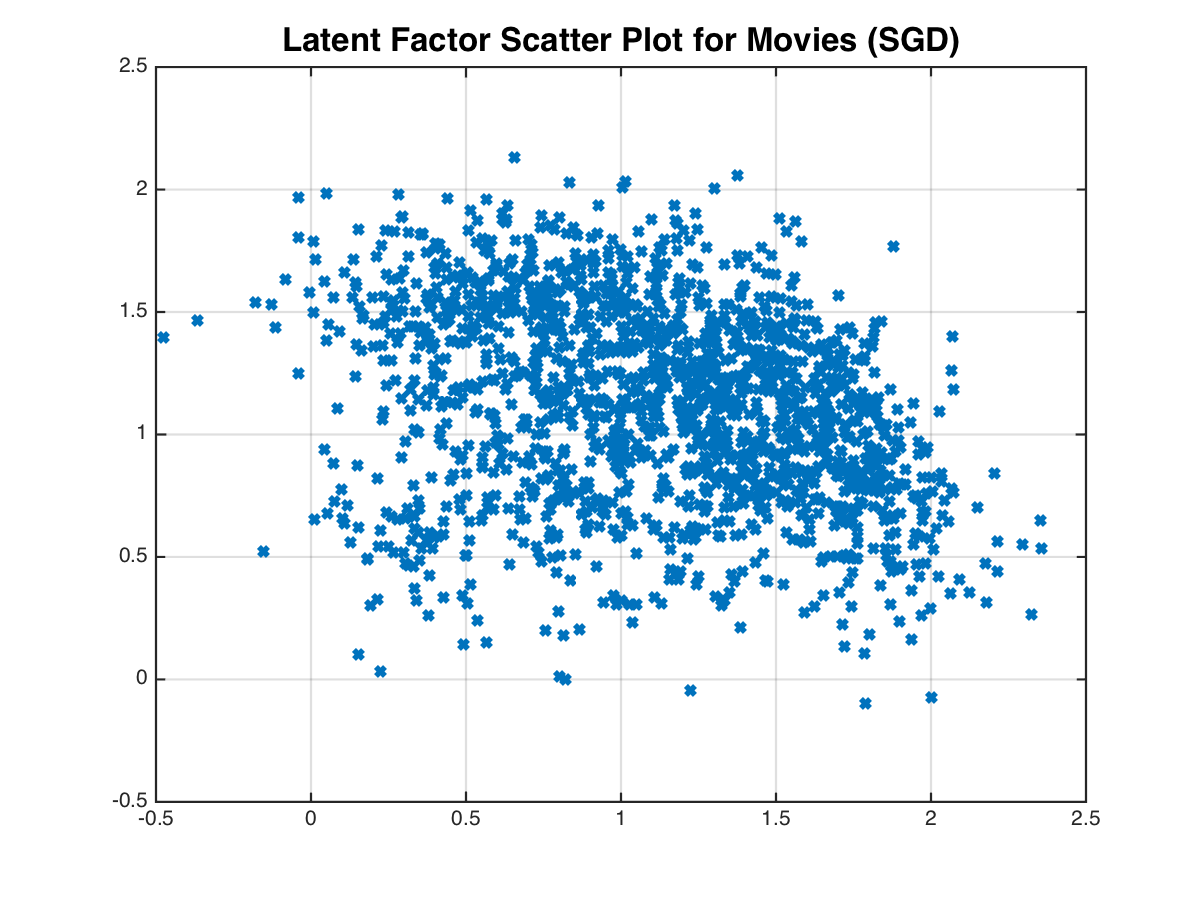
\includegraphics[width=\wiq]{buff5/movs}
		\caption{MovieLens data clustering illustration. Number of latent factors is 2. Trained with SGD, used plain model. This is the latent factor values for all 1682 movies. No clusters can be spotted. This points out that 2 factors are too small to capture the characteristics.}
		\label{5}		
	\end{figure}
	\begin{figure}[H]
		\centering		
		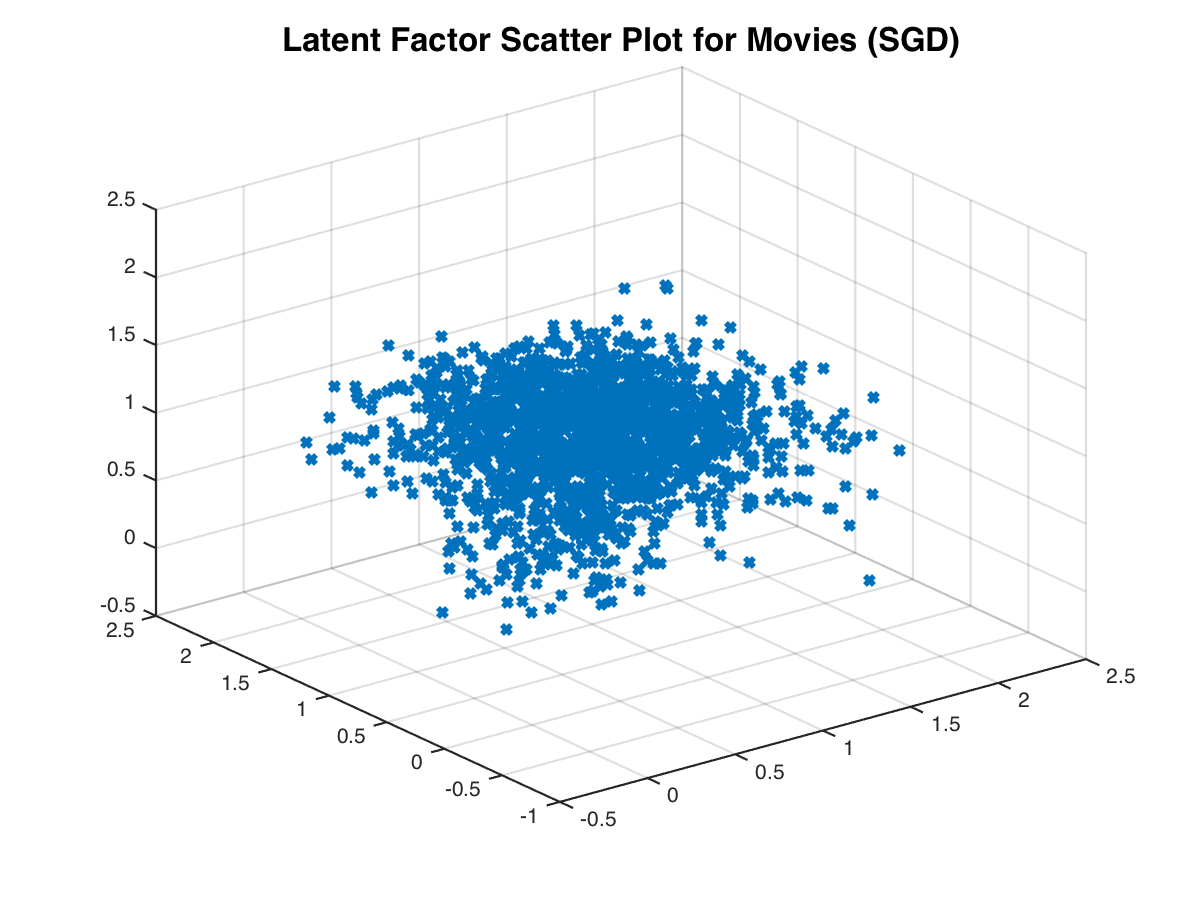
\includegraphics[width=\wi]{buff5/movs2}
		\caption{MovieLens data clustering illustration. Number of latent factors is 3. Trained with SGD, used plain model. This is the latent factor values for all 1682 movies. No clusters can be spotted. This points out that 3 factors are too small to capture the characteristics.}
		\label{5}		
	\end{figure}
	\begin{figure}[H]
		\centering		
		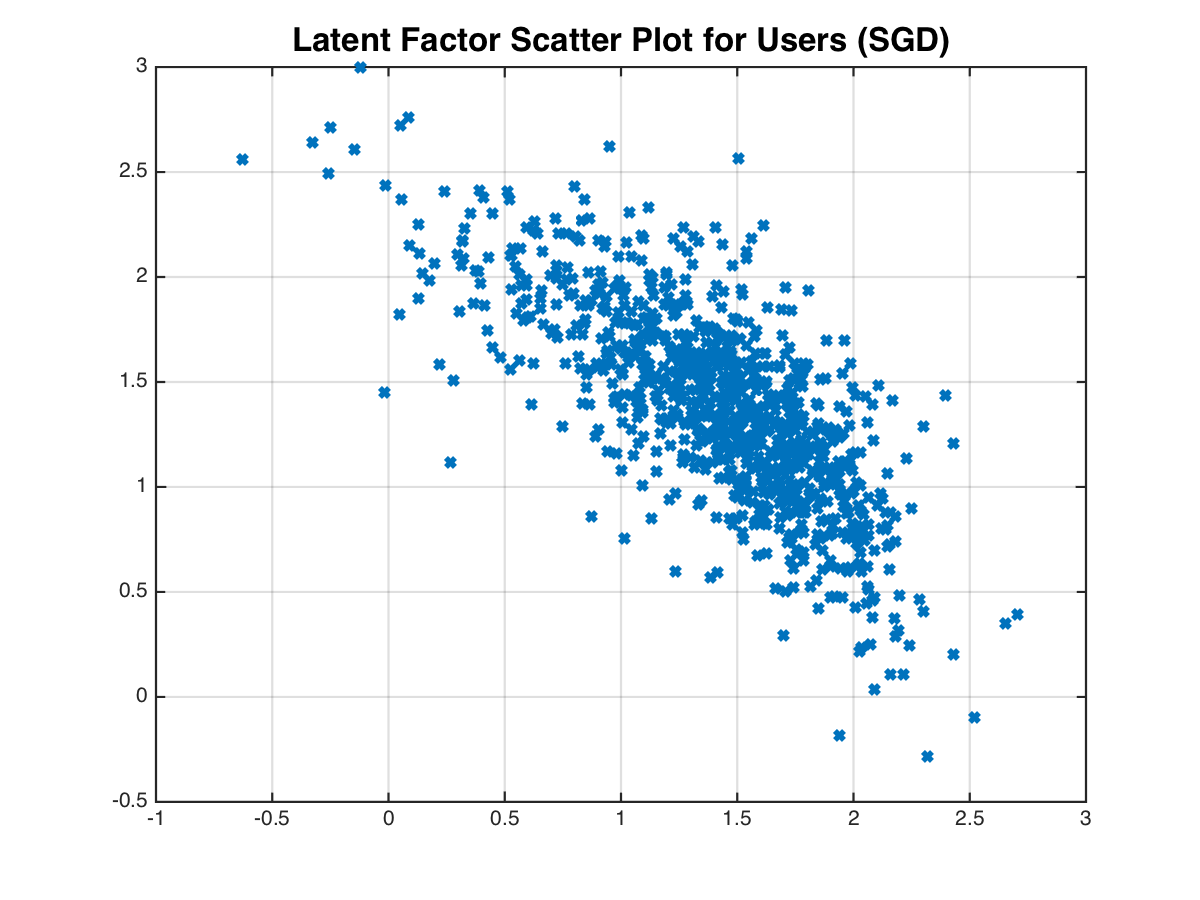
\includegraphics[width=\wi]{buff5/users}
		\caption{MovieLens data clustering illustration. Number of latent factors is 2. Trained with SGD, used plain model. This is the latent factor values for all 943 users. No clusters can be spotted. This points out that 2 factors are too small to capture the characteristics.}
		\label{5}		
	\end{figure}
	\begin{figure}[H]
		\centering		
		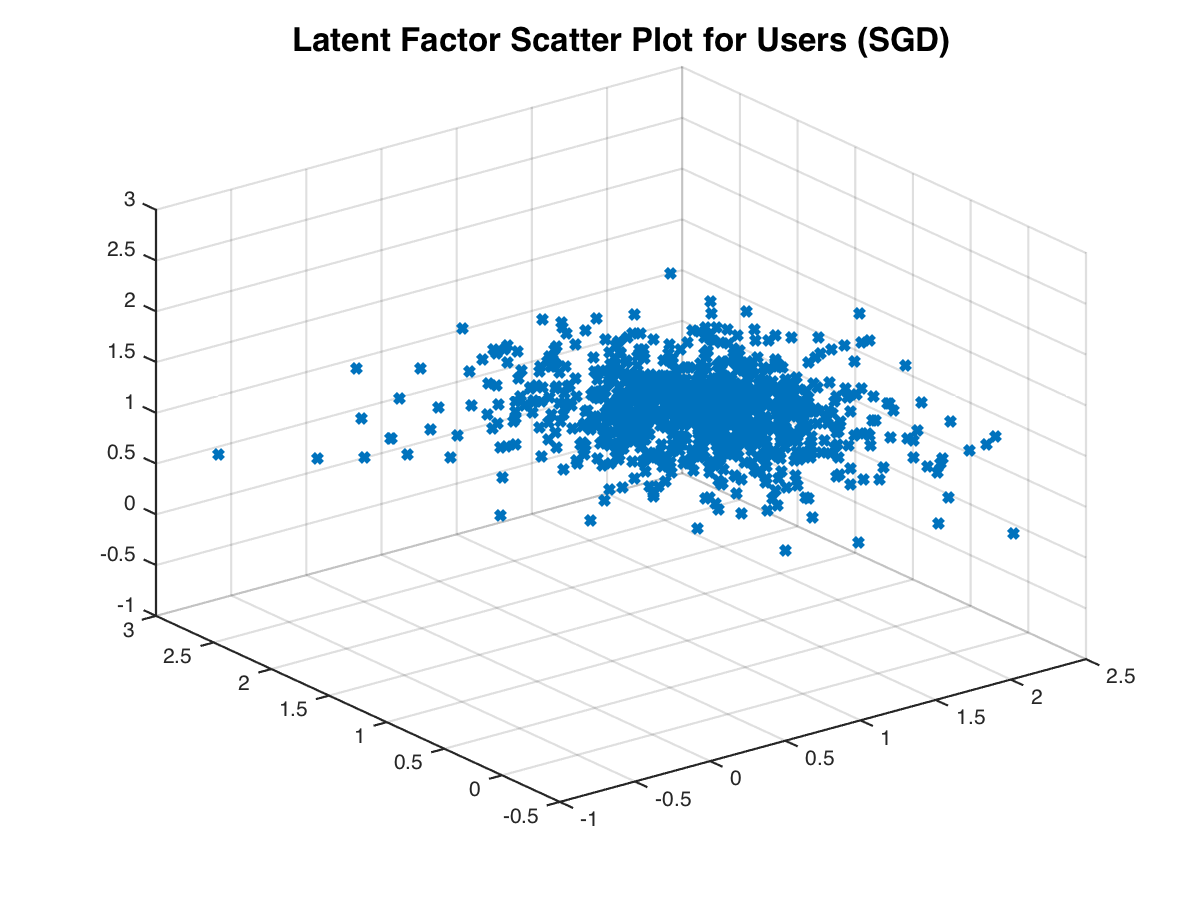
\includegraphics[width=\wi]{buff5/users2}
		\caption{MovieLens data clustering illustration. Number of latent factors is 3. Trained with SGD, used plain model. This is the latent factor values for all 943 users. No clusters can be spotted. This points out that 3 factors are too small to capture the characteristics.}
		\label{5}		
	\end{figure}


	\begin{figure}[H]
		\centering		
		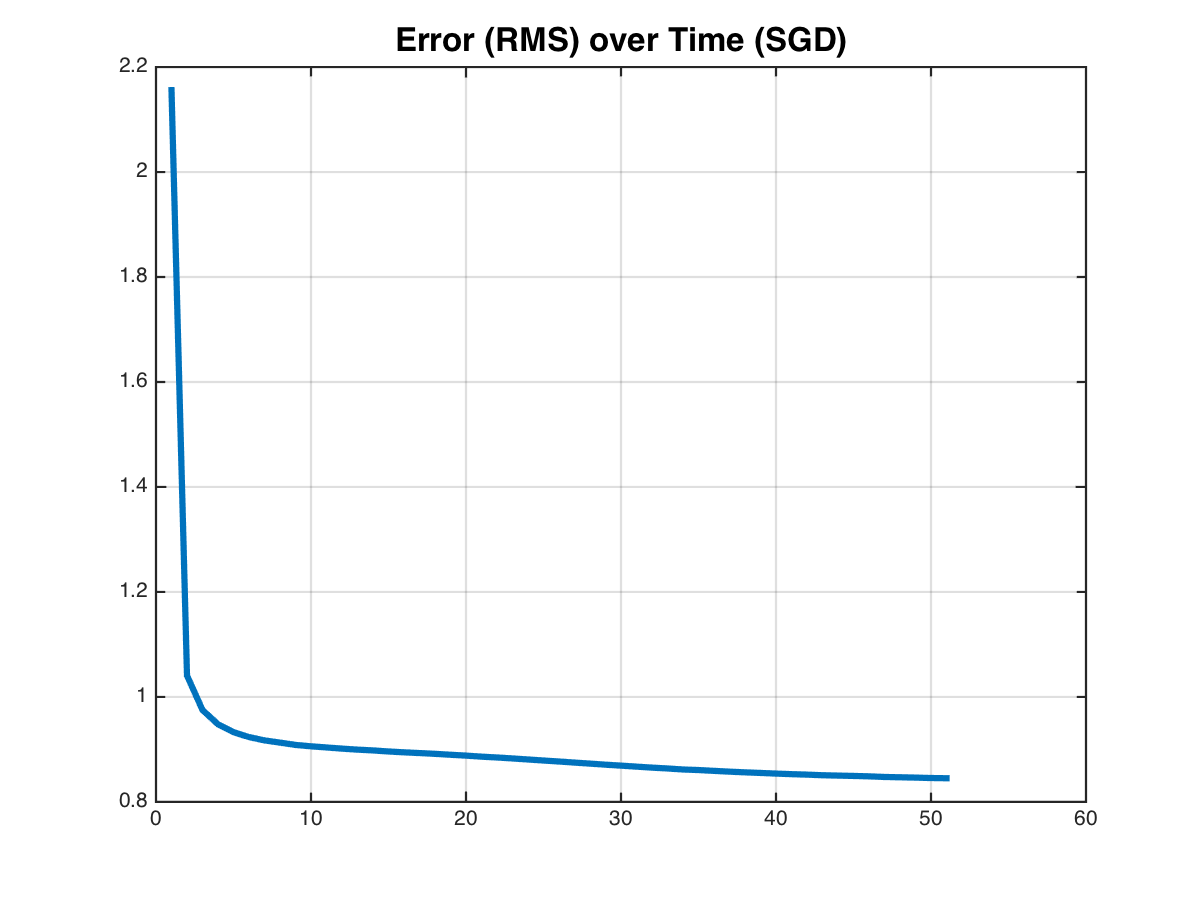
\includegraphics[width=\wi]{buff5/3_on_reg01}
		\caption{MovieLens data illustration. Plot of root mean square errors versus epochs using SGD, used plain model. Where epoch is one iteration through whole dataset.}
		\label{5}		
	\end{figure}
	\begin{figure}[H]
		\centering		
		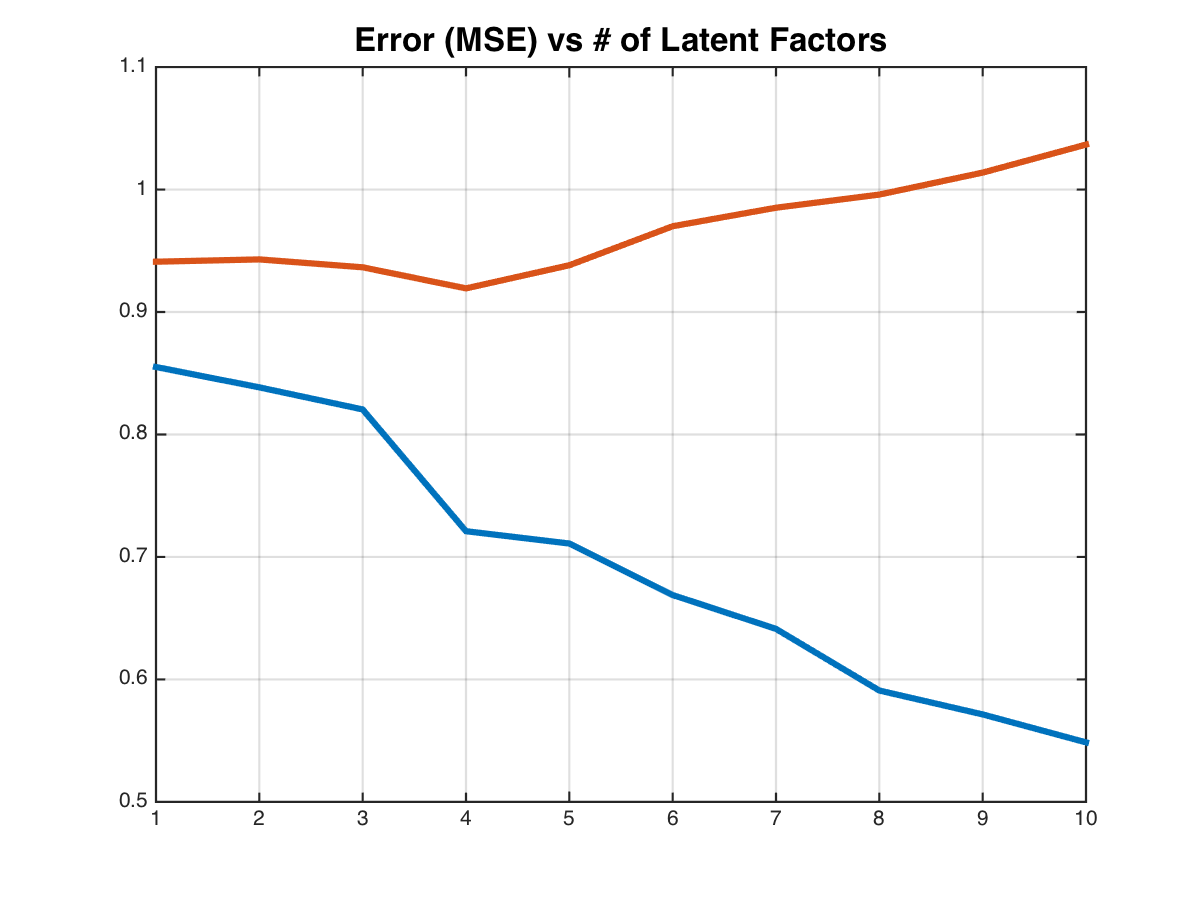
\includegraphics[width=\wi]{buff5/l_sgd}
		\caption{MovieLens data illustration. This plot demonstrates how error on training (blue) and test (red) data changes according to number of latent factors when the model is trained with SGD. }
		\label{5}		
	\end{figure}	
	\begin{figure}[H]
		\centering		
		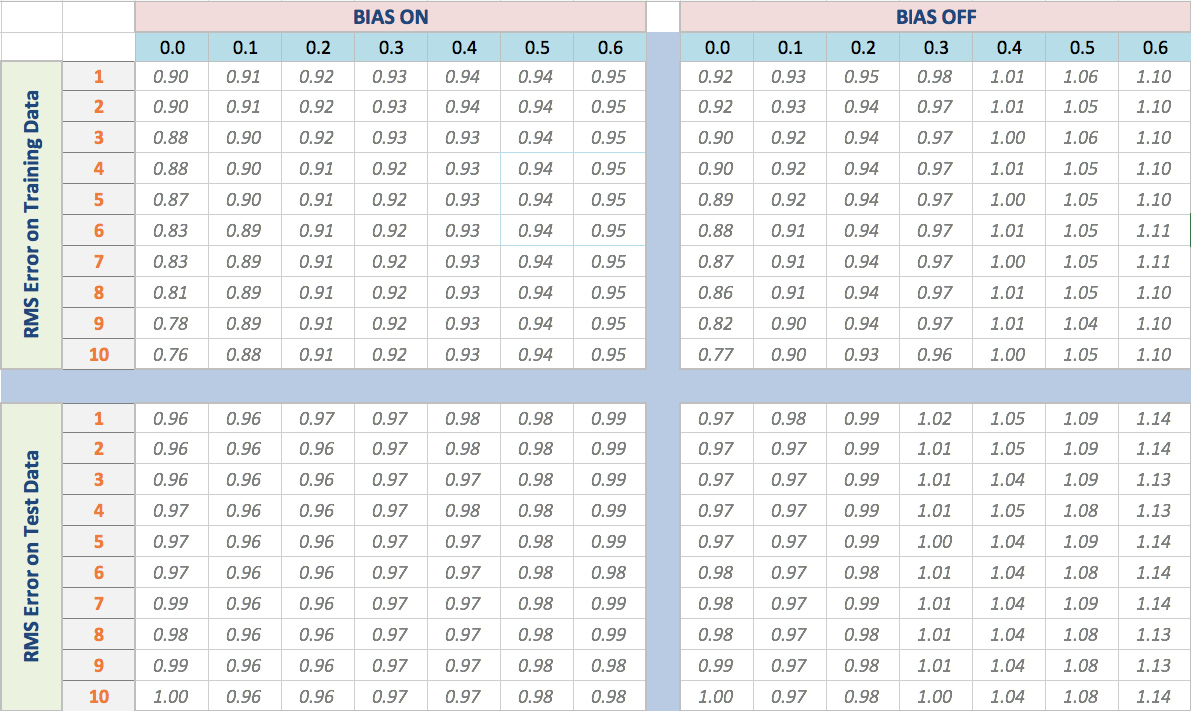
\includegraphics[width=0.85\columnwidth]{buff5/l_reg_err}
		\caption{MovieLens data illustration. Table  of root mean square errors on training and test data according to chosen number of latent factor [1-10], regularization coefficient [0.0-0.6] and bias condition {0,1}. When bias is set on the bias terms \textit{(described in "Approach" section)} are included in the training of the model and vice versa. Bias terms in the model indicate a slight enhancement.}
		\label{5}		
	\end{figure}
		
	\begin{figure}[H]
		\centering		
		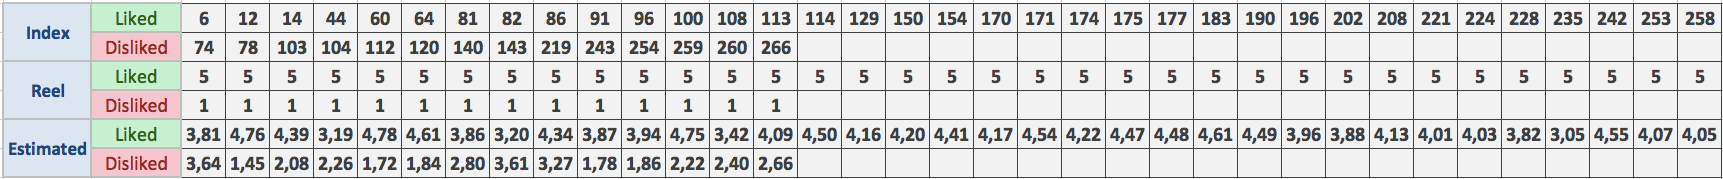
\includegraphics[width=\columnwidth]{buff5/recom_val}
		\caption{In this table we show the estimated ratings for favourite (rated five stars) and disliked (rated one star) movies of a random user. Index rows contain movie ids rather than names.}
		\label{5}		
	\end{figure}
	
	\vspace{15mm}
	
	\begin{figure}[H]
		\centering		
		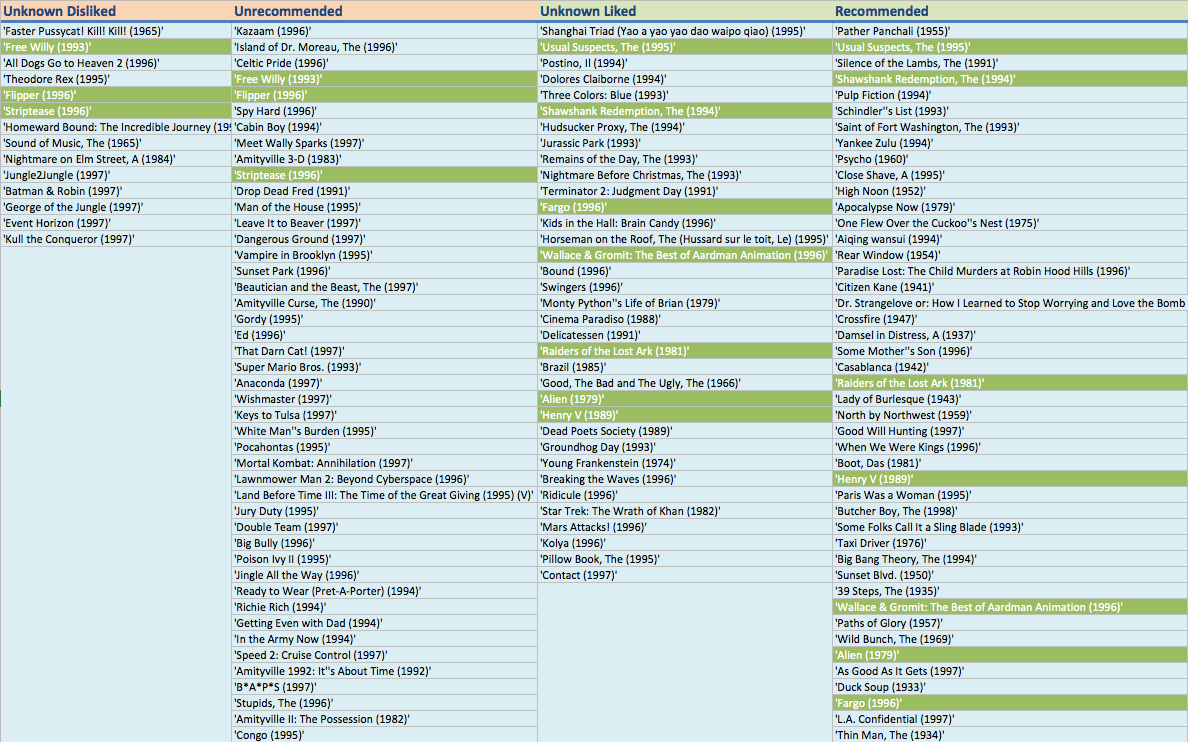
\includegraphics[width=1\columnwidth]{buff5/recom}
		\caption{In this table \textbf{Unkown Disliked} column contains the movies given one star by a random user. They are \textit{unkown} to system becuse movies are from test set. Similarly, \textbf{Unknown Liked} column contains the movies given five stars by that user. \textbf{Recommended} column contains the movies that we estimated highest ratings for. In like manner, \textbf{Unrecommended} column contains the movies that we estimated lowest ratings for.}
		\label{5}		
	\end{figure}
	\clearpage

\section{Appendices}

	See the source code online at \url{https://github.com/oeken/cathar} \\ 
		
	\noindent \large \textbf{script\_1.m}	
	\lstinputlisting[language=Matlab,basicstyle=\footnotesize,numbers=left,frame=single]{../code/script_1.m}
	\vspace{5mm}
	
	\noindent \large \textbf{sgd.m}	
	\lstinputlisting[language=Matlab,basicstyle=\footnotesize,numbers=left,frame=single]{../code/sgd.m}
	\vspace{5mm}

	\newpage
	\noindent \large \textbf{als.m}	
	\lstinputlisting[language=Matlab,basicstyle=\footnotesize,numbers=left,frame=single]{../code/als.m}
	\vspace{5mm}
	
	\noindent \large \textbf{has\_converged.m}	
	\lstinputlisting[language=Matlab,basicstyle=\footnotesize,numbers=left,frame=single]{../code/has_converged.m}
	\vspace{5mm}
	
	\noindent \large \textbf{compute\_error.m}	
	\lstinputlisting[language=Matlab,basicstyle=\footnotesize,numbers=left,frame=single]{../code/compute_error.m}
	\vspace{5mm}
	
	\noindent \large \textbf{to\_instances.m}	
	\lstinputlisting[language=Matlab,basicstyle=\footnotesize,numbers=left,frame=single]{../code/to_instances.m}
	\vspace{5mm}
	
	\noindent \large \textbf{to\_matrix.m}	
	\lstinputlisting[language=Matlab,basicstyle=\footnotesize,numbers=left,frame=single]{../code/to_matrix.m}
	\vspace{5mm}
\end{document}